%%%%%%%%%%%%%%%%%%%%%%%%%%%%%%%%%%%%%%%% Klasse Festlegen
\documentclass[Bachelor,BIF,german,IEEE]{BASE/twbook} 
%%%%%%%%%%%%%%%%%%%%%%%%%%%%%%%%%%%%%%%% Verwendete Packages
\usepackage[utf8]{inputenc} % Zeichen-Enkodierung (evtl. Abweichungen für Apple)
\usepackage[T1]{fontenc}    % Zeichen-Enkodierung
\usepackage{blindtext}      % Platzhaltertexte
\usepackage{minted}         % Darstellung von Code
\usepackage{comment}        % Auskommentieren von ganzen Passagen
\usepackage{csquotes}
\usepackage{algorithm}      % Umgebung f Algorithmen
\usepackage[noend]{algpseudocode}
% Weitere Packages
\usepackage{graphicx}
\usepackage{tabularx}
\usepackage{hyperref}
\usepackage{enumitem}
%%%%%%%%%%%%%%%%%%%%%%%%%%%%%%%%%%%%%%%% Zitierstil
\usepackage[backend=biber, style=ieee]{biblatex}            % LaTeX definierter IEEE- Standard
\addbibresource{Literatur.bib}                              % Literatur-File definieren
%%%%%%%%%%%%%%%%%%%%%%%%%%%%%%%%%%%%%%%% Deckblatt
\title{Technologische Effizienz im Web:\\Einsparung von Ressourcen und Reduzierung der CO$_2$-Emissionen durch Optimierung}

\author{Artjom Moisejev}
\studentnumber{2110257055}

\supervisor{Markus Holzer, MSc}

\place{Wien}
%%%%%%%%%%%%%%%%%%%%%%%%%%%%%%%%%%%%%%%% Danksagung/Kurzfassung/Schlagworte
\kurzfassung{Die vorliegende Bachelorarbeit untersucht den Einfluss der Webtechnologien, die auf österreichischen Webseiten eingesetzt werden, auf CO$_2$-Emissionen und das Potenzial zur Energieeinsparung. 
Durch den Einsatz eines, speziell für diese Forschung entwickelten, Webcrawlers wurden Performance-Daten gesammelt, in Google Sheets verwertet und anschließend in MATLAB analysiert. 
Die Analyse umfasst 3246 Webseiten und bestätigt das Bild des \glqq verschlafenen Österreichs\grqq . 
Es zeigt ein immenses Potential für Verbesserungen, sowohl in der Aktualität der verwendeten Software, als auch in Bereichen der Performance und Energieeffizienz. 
Die größte Schwankungsbreite lag bei WordPress-Webseiten, was das Potenzial für Extremfälle bei No-Code-Plattformen unterstreicht und die Betreiber in die Verantwortung zieht, die eigene Webpräsenz zu optimieren.
Aufgrund dieser Erkentnisse empfiehlt die vorliegende Arbeit eine bewusste Auswahl und Implementierung von Web-Technologien, kombiniert mit effektiven Optimierungsstrategien, um die Umweltauswirkungen im digitalen Raum zu senken. 
Dabei liegt eine besondere Empfehlung für die Benutzer von WordPress und anderen No-Code Plattformen, zumindest auf die Mediengrößen und die Anzahl der Drittanbieter-Software zu achten, da in diesen Bereichen die größten Potentiale zur Einsparung von Energie und CO$_2$-Emissionen liegen.}
\schlagworte{Web-Technologien, CO$_2$-Emissionen, Energieeffizienz, Webcrawler, Leistungsoptimierung, ökologischer Fußabdruck, nachhaltige IT, Datenanalyse, Optimierung von Webseiten}
\outline{This bachelor thesis examines the influence of web technologies used on Austrian websites on CO$_2$ emissions and the potential for energy savings. 
Using a web crawler specially developed for this research, performance data was collected, used in Google Sheets and then analyzed in MATLAB. 
The analysis covers 3246 websites and confirms the image of \glqq sleepy Austria\grqq . 
It shows immense potential for improvement, both in the up-to-dateness of the software used, as well as in performance and energy efficiency. 
WordPress websites showed the greatest variation, which underlines the potential for extreme cases with no-code platforms and makes operators responsible for optimizing their own web presence.
Based on these findings, this paper recommends a conscious selection and implementation of web technologies, combined with effective optimization strategies to reduce the environmental impact in the digital space. 
A particular recommendation for users of WordPress and other no-code platforms is to at least pay attention to the media sizes and the number of third-party software, as these are the areas with the greatest potential for saving energy and CO$_2$ emissions.}
\keywords{Web technologies, CO$_2$ emissions, energy efficiency, web crawler, performance optimization, ecological footprint, sustainable IT, data analysis, website optimization}

\acknowledgements{Die erste und größte Danksagung spreche ich an meine heiß- und viel-geliebte Mercedes aus. Sie war nicht nur die größte positive Wendung meines Lebens, sondern hat mir diesen Traum vom IT-Studium überhaupt erst ermöglicht. Ihre Liebe und Fürsorge, sowie ihr Glaube an mich, mit einhergehender dauerhaften Unterstützung, sei es seelisch, emotional, physisch oder finanziell, haben mir das Durchhaltevermögen geschenkt, das Studium und diese Bachelorarbeit nicht nur durchzustehen, sondern auf höchstem Niveau auskosten und für persönlichen Wachstum zu nutzen.\newline

\noindent Gefolgt, nach meiner besseren Hälfte, findet sich immer mein bester Freund Maciej, der oft meine einzige Auszeit und Ausgleich darstellte, zum Studium selbst, zum Schreiben dieser Arbeit und zur beruflichen Tätigkeit. Seine Loyalität und Gastfreundschaft gaben mir den stabilen Halt in dieser stürmischen Zeit und spielten somit eine grundlegende Rolle auf meinem Weg. An dieser Stelle auch ein Dank an seine Mutter Krystyna, die mir immer ein Gefühl des Willkommen-seins vermittelte und stets ein paar nette Worte für mich fand. Und natürlich auch an ihren Kater Jakus.\newline

\noindent Ein weiterer wichtiger Grundpfeiler meines Werdegangs ist Dominik, mein Studienkollege und Gründer-Partner des IT-Unternehmens 27vier Development. Mit ihm an meiner Seite war ich stets beflügelt, das Beste aus dem Studium und dieser Bachelorarbeit zu machen, um das Wissen wieder in das gemeinsame Unternehmen zu investieren. Mit diesem Antrieb gelangen mir die Extrameilen für die hohe Qualität und den breiten Umfang dieser Arbeit.\newline

\noindent Weiters bedanke ich mich bei allen anderen Menschen, die mich auf dem Weg unterstützt haben: Meinen Betreuer MSc Markus Holzer, für die Begutachtung und Betreuung dieser Arbeit; Shane, für seinen Glauben an mich; meine beiden Brüder Patrick und Mark Moisejev, sowie meine Schwester Diana Moisejev, für die kleinen Auszeiten an Feiertagen und Ferien.\newline
\clearpage
\noindent Abschließend möchte ich ein Wort der Trauer aussprechen für all die anderen interessanten Bachelorthemen \dag , die ich gerne bearbeitet hätte, aber letztendlich den Webcrawler gewählt habe. RIP 
\begin{itemize}
    \item Plan A: CO$_2$ Einsparung durch Performance Optimierung von Webseiten (Erledigt)
    \item Plan A$_1$: Betriebssysteme analysieren: staatliche Ämter, ÖBB, etc. (Linux > Windows)
    \item Plan B: B-Side (altes Projekt für Musiker-Plattform)
    \item Plan C: ChatGPT (Auswirkungen auf Lernfähigkeit - Mails schreiben, Coden verlernen)
    \item Plan G: Grafische Turing Maschine/Automat mit Pixel, statt Band (Ähnlich wie Game of Life von John Conway \dag )
    \item Plan Q: Quadtrees untersuchen (Travelling Salesman Problem?)
    \item Plan O: OpenGL - irgendwas mit Shadern machen
    \item Plan W: Internetwerbung (Wieso das Konzept zum Scheitern verurteilt ist)
\end{itemize}
}
\setListingsAndAcronyms % Definition der Namen für Quellcodeverzeichnis 
%%%%%%%%%%%%%%%%%%%%%%%%%%%%%%%%%%%%%%%% Ende des Headers
%%%%%%%%%%%%%%%%%%%%%%%%%%%%%%%%%%%%%%%% Beginn des Dokuments
\begin{document}
%%%%%%%%%%%%%%%%%%%%%%%%%%%%%%%%%%%%%%%% 
\maketitle
%%%%%%%%%%%%%%%%%%%%%%%%%%%%%%%%%%%%%%%% Beginn des Inhalts
% ------------------------------------------------------------------------------------------
% KAPITEL 1 - Einleitung
\chapter{Einleitung}

\section{Hintergrund des Problems}
\noindent Das World-Wide-Web und die damit einhergehende digitale Revolution haben die Art und Weise wie wir kommunizieren, arbeiten und leben, grundlegend verändert.
Diese Technologien sind jedoch nicht ohne ökologische Kosten.
Es wird geschätzt  \cite{ICT21}, dass die \ac{IKT} ca. 1,8 \% - 2,8 \% der weltweiten Treibhausgasemissionen im Jahr 2020 ausmachten, mit Schätzungen der Emissionen der \ac{IKT}, die zwischen 0,8 und 2,3 GtCO$_2$ variierten.
Die höchsten Schätzungen setzen den Anteil der \ac{IKT} an den weltweiten Emissionen auf etwa 6,3 \% fest, wobei aktuellere Bewertungen ein Best Case Szenario von etwa 1,5 \% als realistisch betrachten.
Vor dem Hintergrund des Klimawandels wird die Notwendigkeit, den ökologischen Fußabdruck digitaler Technologien zu reduzieren, immer dringlicher. An anderer Stelle  \cite{GEU30} zeigen Prognosen für 2030, dass der Trend des steigenden Energiebedarfs sich nicht nur fortsetzen wird, mit einem Wachstum von 2,8 \% - 3,4 \%, sondern auch nur zu 29 \% im Best Case und 16 \% im Worst Case, von erneurbaren Energien betrieben sein wird.

\section{Problemstellung}
\noindent Die voranschreitende Digitalisierung öffnet für User und Unternehmen neue Möglichkeiten und macht es für alle einfacher, eine Webpräsenz aufzubauen. Ein besonderes Augenmerk liegt auf dem stetig wachsenden Marktanteil von WordPress, der mittlerweile auf 43 \% angestiegen ist  \cite{WP42}, aber auch auf anderen No-Code-Lösungen (wie Wix, SquareSpace, Webflow, etc.), die aufgrund ihrer Einfachheit und Zugänglichkeit immer attraktiver werden.
Diese Entwicklungsplattformen ermöglichen es Nutzern ohne tiefe Fachkenntnisse, Webseiten zu erstellen und zu verwalten. Jedoch kann das Fehlen von technischem Wissen in vielen Fällen zu suboptimalen Lösungen führen, die nicht nur ineffizient und energieintensiv sein können, sondern auch den Gebrauch von proprietärer Black-Box-Software machen und somit dem Webseitenbesitzer nur wenige Möglichkeiten bieten, die Effizienz zu steigern. Insbesondere die übliche Praxis von Unternehmen, gewinnorientierte Entscheidungen zu treffen, wie aggressive Sparmaßnahmen, sich für die günstigsten Anbieter zu entscheiden oder ein Übermaß an Diensten von Drittanbietern zu nutzen, birgt ein erhebliches Potential für Energieverschwendung bzw. Einsparungspotential  \cite{CIO24}. Dass es einen signifikanten Unterschied in den CO$_2$-Emissionen zwischen verschiedenen Plattformen gibt, zeigte die Studie  \cite{SM22}, bei der moderne Plattformen, wie YouTube, Facebook, Netflix und TikTok, hinsichtlich ihrer CO$_2$-Emissionen untersucht wurden. Die Tatsache, dass moderne Hardware leistungsfähiger und verzeihender gegenüber ressourcenintensiven Prozessen ist  \cite{HW20}, verstärkt dieses Problem weiter und trägt dazu bei, dass Webseiten oft viel mehr Ressourcen verbrauchen als notwendig, was sowohl die direkten als auch die indirekten Umweltauswirkungen erhöht. Selbst unter professionellen Entwicklern herrscht Unwissen bezüglich Energy Patterns  \cite{EnP24}, welches auf Energiesparpotenziale in der zugrunde liegenden Software der Plattformen selbst hindeuten kann.

\section{Ziel der Arbeit}
\noindent Angesichts der dringenden Notwendigkeit, die Auswirkungen des Klimawandels zu bekämpfen, ist es entscheidend, die Problemstellung rund um den Energieverbrauch und die damit verbundenen CO$_2$-Emissionen von Webseiten und Web-Apps zu analysieren. Die Herausforderung besteht darin, effektive Lösungsansätze zu identifizieren, die nicht nur die ökologische Nachhaltigkeit fördern, sondern auch die breite Palette von Usern einschließen – von Einzelpersonen ohne technischen Hintergrund bis hin zu großen Unternehmen. Durch die Entwicklung und Anwendung von nachhaltigeren Web-Technologien und Optimierungsstrategien  \cite{GSF24} kann ein bedeutender Beitrag zur Reduzierung des digitalen ökologischen Fußabdrucks geleistet werden.
Die vorliegende Arbeit zielt darauf ab, den Einfluss von Web-Technologien und Optimierungsstrategien auf den Energieverbrauch und die CO$_2$-Emissionen von Webseiten zu untersuchen, um Einsparungspotenziale aufzuzeigen.
Durch die Analyse verschiedener Webseiten soll herausgefunden werden, welche Technologien und Methoden sich positiv auf die Umweltbilanz auswirken und somit den digitalen Raum umweltfreundlicher gestalten und welche nicht.
Dieses Wissen soll als Grundlage dienen, um Richtlinien und Best Practices für die Entwicklung nachhaltiger Web-Anwendungen zu formulieren, oder vorhandene Forschung zu stützen und somit einen Beitrag zur Bewältigung der ökologischen Herausforderungen unserer Zeit zu leisten.

\section{Forschungsfrage und Hypothesen}
Die zentrale Forschungsfrage dieser Arbeit lautet: \glqq Inwiefern korrelieren bestimmte Web-Technologien und Optimierungen mit dem Energieverbrauch und den CO$_2$-Emissionen von Webseiten?\grqq{} Diese Frage zielt darauf ab, die Beziehung zwischen der technischen Umsetzung von Webseiten und ihren Umweltauswirkungen zu verstehen.\newline

\section{Hypothesen}
\begin{itemize}
    \item Hypothese 1: Es besteht eine signifikante Korrelation zwischen der Verwendung moderner Web-Technologien (wie Frontend-Frameworks, Bibliotheken, \ac{CMS}, etc.) und einer Reduzierung der CO$_2$-Emissionen von Webseiten.
    \item Hypothese 2: Webseiten, die für Performance und Effizienz optimiert sind (z.B. durch die Minimierung des Datenverkehrs und effiziente Ressourcennutzung), haben im Vergleich zu weniger optimierten Webseiten einen geringeren ökologischen Fußabdruck.
\end{itemize}

\noindent Diese Hypothesen sollen durch den Einsatz eines selbst entwickelten Webcrawlers überprüft werden, der relevante Daten und Metriken von einer Vielzahl von Webseiten sammelt und analysiert. Die Ergebnisse dieser Analyse werden aufzeigen, inwieweit Webentwickler und -designer durch gezielte Technologie- und Optimierungswahl zur Reduzierung des CO$_2$-Fußabdrucks beitragen können.

\clearpage   


% ------------------------------------------------------------------------------------------
% KAPITEL 2 - Methodik - 20%
\chapter{Methodik}

\noindent Die Forschungsfrage und die Hypothesen sollen durch den kombinierten Einsatz eines selbst entwickelten Webcrawlers, der die Datensammlung ausführt, Google Sheets als Speicher der Daten und MATLAB für die Analyse der gesammelten Daten, überprüft werden. Der Crawler ermöglicht die automatisierte Sammlung der Daten und die Analyse der Webseiten hinsichtlich ihrer Performance, des Technologieeinsatzes und der Optimierungsstrategien einer breiten Palette von Webseiten. Die Ergebnisse dieser Analyse werden in Google Sheets gesammelt und gesäubert. Anschließend werden die Verarbeitung und Darstellung der Daten in MATLAB durchgeführt, um aufzuzeigen, inwieweit Webentwickler und -designer durch gezielte Technologie- und Optimierungswahl zur Reduzierung des CO$_2$-Fußabdrucks beitragen können.

\section{Forschungsdesign}
Das Forschungsdesign orientiert sich an einer quantitativen Methodologie, um objektiv messbare Daten über den Zusammenhang zwischen Web-Technologien, Optimierungsstrategien und deren Auswirkungen auf den Energieverbrauch sowie die damit verbundenen CO$_2$-Emissionen zu erfassen. Die Entwicklung und Nutzung eines Webcrawlers als zentrales Instrument dieser Forschung ermöglicht es, Daten in großem Umfang zu sammeln und damit eine solide Datenbasis für die Analyse zu schaffen. Diese Methodik erlaubt eine objektive, effiziente und durch die Open-Source-Veröffentlichung des Quellcodes, eine reproduzierbare Datenerhebung, wodurch die Validität und Zuverlässigkeit der Forschungsergebnisse erhöht wird.

\section{Datenerhebung}
Der Kern der Datenerhebung liegt in der Programmierung und dem Einsatz des Webcrawlers. Dieser Crawler wird konfiguriert, um spezifische Daten von einer Vielzahl von Webseiten zu extrahieren, darunter:

\begin{itemize}
    \item Performance-Metriken (z.B. Ladezeiten, Menge heruntergeladener Daten)
    \item Verwendete Web-Technologien und Frameworks (z.B. React, Angular)
    \item Implementierte Optimierungsstrategien (z.B. Minifizierung von Code\footnote{Verkleinerung des Quellcodes \cite{MJS24}}, Bildoptimierung)
\end{itemize}

\noindent Bei der Datenerhebung werden die Ergebnisse vollautomatisch in Google Sheets hochgeladen, um daraufhin analysiert und verwertet zu werden. Die Auswahl der zu analysierenden Webseiten wurde so getroffen, dass sie ein breites Spektrum an Anwendungstypen, Branchen und Technologieeinsätzen abdeckt. Dies stellt sicher, dass die Ergebnisse der Studie generalisierbar und auf verschiedene Kontexte anwendbar sind.

\section{Datenanalyse}
Die Datenanalyse zielt darauf ab, Muster und Korrelationen zwischen den eingesetzten Technologien, den Optimierungsstrategien und den Performance-Metriken mithilfe von MATLAB zu identifizieren. Anhand einer eigenen Score-Berechnung werden Kalkulationen gemacht, um für jede untersuchte Webseite Energieverbrauchs- und CO$_2$-Emissionsschätzungen auszurechnen. Dabei werden verschiedene Diagramme und Tabellen erstellt, um die Verteilungen visuell darzustellen. Um Mittelwerte und Ausreißer aufzuzeigen werden Boxplots verwendet, wobei für Korrelationen wiederum Streudiagramme zum Einsatz kommen. Die Ergebnisse dieser Analysen werden genutzt, um die aufgestellten Hypothesen zu überprüfen und ein tieferes Verständnis für die Effektivität verschiedener Web-Technologien und Optimierungsansätze in Bezug auf die Reduktion des ökologischen Fußabdrucks zu entwickeln. Weiterhin soll die Auswertung der Daten einen Einblick in den aktuellen Digitalisierungsfortschritt der österreichischen Unternehmen, mit Fokus auf Wien, geben.

\clearpage  


% ------------------------------------------------------------------------------------------
% KAPITEL 3 - Lösung - 50%
\chapter{Entwicklung und Untersuchung}

\section{Entwicklung des Webcrawlers}

\subsection{Konzeption und Zielsetzung}
\noindent Die Entwicklung eines Webcrawlers für die Untersuchung des ökologischen Fußabdrucks von Webseiten und Web-Apps entsprang der Notwendigkeit, eine umfangreiche und objektive Datenbasis zu generieren. Diese Datenbasis sollte Aufschluss darüber geben, inwieweit verschiedene Web-Technologien und Optimierungsstrategien den Energieverbrauch und die CO$_2$-Emissionen beeinflussen können. Die Konzeption des Crawlers war daher von Anfang an darauf ausgerichtet, eine Datenerhebung zu ermöglichen, die sowohl in der Breite (Anzahl der untersuchten Webseiten) als auch in der Tiefe (Vielfalt der erfassten Daten) aussagekräftige Informationen liefert. Das primäre Ziel dieses Projekts war die Sicherstellung, dass der Webcrawler zuverlässig, effizient und in einem mittel-hohem Maße skalierbar entwickelt wird. Hierbei sollten insbesondere folgende Aspekte berücksichtigt werden:

\begin{itemize}
    \item Umfassende Datensammlung: Der Crawler sollte in der Lage sein, eine breite Palette von Webseiten zu besuchen und dabei nur relevante Daten zu sammeln, die für die Bewertung ihres Energieverbrauchs und ihrer CO$_2$-Emissionen erforderlich sind. Dazu gehören technische Spezifikationen, wie der Einsatz von Frameworks und Bibliotheken, sowie Performancedaten.
    \item Präzise Analysefähigkeit: Neben der Sammlung von Daten war es essentiell, dass der Crawler diese Informationen in einem Format bereitstellt, das eine detaillierte Analyse ermöglicht. Dies beinhaltet die Fähigkeit, die Daten so zu strukturieren und zu speichern, dass sie leicht zugänglich, gut analysierbar und vor allem verlässlich konsistent gespeichert werden.
    \item Skalierbarkeit und Effizienz: Angesichts der schieren Menge an Webseiten, die für eine umfassende Analyse erforderlich sind, musste der Crawler auch skalierbar und so effizient in seiner Arbeitsweise sein, wie nur möglich. Dies bedeutet, dass er in der Lage sein sollte, eine große Anzahl von Seiten in einem vertretbaren Zeitrahmen zu verarbeiten, ohne dabei die Genauigkeit oder die Qualität der gesammelten Daten zu beeinträchtigen.
\end{itemize}

\noindent Die Konzeption des Webcrawlers wurde mit dem Bewusstsein vorgenommen, dass die Qualität und Relevanz der gesammelten Daten direkt die Glaubwürdigkeit und Aussagekraft der gesamten Forschungsarbeit beeinflussen. Daher wurde besonderer Wert auf die Auswahl der zu sammelnden Daten, die Architektur des Crawlers und die Strategien zur Datenanalyse gelegt. Durch diesen methodischen Ansatz soll sichergestellt werden, dass die Ergebnisse der Arbeit einen signifikanten Beitrag zum Verständnis und zur Reduzierung des ökologischen Fußabdrucks digitaler Technologien leisten.

\subsection{Technische Spezifikationen}
\noindent Die technische Umsetzung des Webcrawlers basiert auf einer Kombination moderner Technologien und Tools, die zusammenarbeiten, um eine effiziente Datensammlung und -analyse von Webseiten zu ermöglichen. Im Folgenden werden die Schlüsseltechnologien und deren Einsatz im Rahmen dieses Projekts erläutert.

\subsubsection{Node.js}
Node.js \cite{NPM24} bildet die Grundlage des Webcrawlers und wurde aufgrund seiner Leistungsfähigkeit bei der Handhabung asynchroner Operationen und Netzwerkanfragen sowie der Vielfalt an Open-Source-Bibliotheken ausgewählt. Es ermöglicht die schnelle und einfache Entwicklung eines performanten und skalierbaren Crawlers, da es eine umfangreiche Bibliothek von Modulen bietet, die für verschiedene Aspekte des Crawlings selbst, der Datenverarbeitung und der Datensammlung genutzt werden können.

\subsubsection{Cheerio für statische Analyse}
Cheerio \cite{CHEER24} wird eingesetzt, um die heruntergeladenen HTML-Dokumente der Webseiten zu analysieren. Es bietet eine einfache und effiziente Methode, um mit dem DOM der Seite zu interagieren, ähnlich wie jQuery. Durch den Einsatz von Cheerio kann der Crawler spezifische Daten aus dem HTML extrahieren, wie z.B. Meta-Tags, Header, bestimmte Dateinamen und andere Informationen. Diese Fähigkeit ist essenziell, um Daten über den Technologie-Stack, die Implementierung von Optimierungstechniken und die allgemeine Integration und Klassifizierung der verwendeten Web-Technologien zu erfassen.

\subsubsection{Puppeteer und Lighthouse für Performance-Tests}
Puppeteer \cite{PPTR24} dient als Headless Chrome Browser, der es ermöglicht, Webseiten unter realen Bedingungen zu rendern und mit ihnen automatisiert zu interagieren. In Kombination mit Lighthouse \cite{GLH24}, einem von Google entwickelten Tool für die Performance-Analyse von Webseiten und Webanwendungen, ermöglicht Puppeteer die Durchführung detaillierter Performance-Tests. Lighthouse bietet umfassende Berichte über verschiedene Aspekte der Webseiten-Performance, einschließlich der Ladezeit, der Performance-Einsparungspotenziale und des überschüssigen Datenverkehrs. Diese Daten sind entscheidend, um zu bewerten, wie verschiedene Technologien und Optimierungen den Energieverbrauch und die Effizienz von Webseiten beeinflussen.

\subsubsection{CO2.js}
CO2.js \cite{CO2JS24} ist eine Open-Source-Bibliothek der Green Web Foundation und dient zur Schätzung der CO$_2$-Emissionen anhand der übertragenen Datenmenge. Es ermöglicht auch den Abgleich mit einer internationalen Datenbank \cite{GHDB24}, die Hosting-Anbieter auflistet, welche grünen Strom für ihre Dienstleistungen verwenden. Dies hilft bei der Einschätzung der CO$_2$-Emissionen und gibt einen weiteren Einblick in den aktuellen Stand der Verbreitung von grünem Hosting.

\subsubsection{Google Sheets für Datensammlung}
Google Sheets dient als zentrale Plattform für die Speicherung und erste Verarbeitung der gesammelten Daten. Die Verwendung von Google Sheets ermöglicht eine flexible und online zugängliche Methode zur Organisation der Daten, die von verschiedenen Webseiten gesammelt wurden. Außerdem bietet es eine einfache Benutzeroberfläche und die wichtigsten Werkzeuge auf einem Fleck, anders als bei der Microsoft-Alternative MS Excel, was den zeitlichen Aufwand der Forschung verzögern würde.

\subsubsection{Google API zur Kommunikation mit Google Sheets}
Um die Interaktion zwischen dem Webcrawler und Google Sheets zu ermöglichen, wird die Google Sheets API \cite{GAPI24} verwendet. Diese API ermöglicht es dem Crawler, automatisch Daten in Google Sheets einzufügen, zu aktualisieren oder zu lesen. Durch die Programmierung spezieller Skripte kann der Crawler effizient mit der Google Sheets-Datenbank kommunizieren, was die manuellen Dateneingaben eliminiert und den gesamten Prozess der Datensammlung und -analyse weiter automatisiert.

\subsubsection{MATLAB}
MATLAB \cite{MAL24} wird verwendet, um genauere mathematische Analysen und daraus resultierende Ergebnisse/Daten visuell auszuarbeiten. Durch die exakte Genauigkeit und die Möglichkeit, die erhobenen Daten flexibel zu kombinieren sowie darzustellen, erhält MATLAB eine zentrale Rolle in der Auswertung und Analyse der gesammelten Daten. Weiterhin wird durch die Offenlegung des verwendeten MATLAB-Codes die Reproduzierbarkeit dieser Forschung weiter verstärkt.\newline

\noindent Die Kombination dieser Technologien ermöglicht die Entwicklung eines leistungsfähigen Webcrawlers, der nicht nur umfangreiche Daten von einer Vielzahl von Webseiten sammeln, sondern auch tiefgreifende Einblicke in deren Performance und ökologischen Fußabdruck liefern kann. Durch die Nutzung von Node.js, Cheerio, Puppeteer, Lighthouse, CO2.js und der Google Sheets API kann der Crawler komplexe Aufgaben der Datensammlung und -analyse effizient bewältigen und wertvolle Informationen für die Forschung bereitstellen. Die anschließende Auswertung durch MATLAB ermöglicht eine präzise und zuverlässige Darstellung der Daten.

\subsection{Konfiguration und Funktionsweise des Webcrawlers}
\noindent Ein wesentlicher Aspekt bei der Entwicklung des Webcrawlers ist seine Flexibilität in Bezug auf die Datenspeicherung. Standardmäßig ist der Crawler so konfiguriert, dass er die gesammelten Daten in Google Sheets einfügt, was eine einfache und effiziente Möglichkeit bietet, die Ergebnisse in Echtzeit zu überwachen und zu analysieren. Diese Konfiguration eignet sich besonders für Teams, die an der Datensammlung beteiligt sind, da der Zugriff und die Kollaboration dadurch erleichtert wird. Außerdem ermöglicht die zentrale Online-Speicherung, den Betrieb von mehreren Crawlern gleichzeitig, von verschiedenen Geräten aus. Dies war jedoch bei der Datensammlung für diese Arbeit nicht der Fall.
Für Anwender, die eine lokale Lösung bevorzugen oder eine Offline-Analyse der Daten durchführen möchten, bietet der Crawler eine alternative Konfiguration. Durch Setzen der Flag \texttt{{-}{-}local}, bei der Ausführung des Crawlers, können die Daten stattdessen in eine lokale CSV-Datei geschrieben werden. Diese Option erhöht die Flexibilität des Crawlers erheblich, da User ohne Zugang zu Google Sheets oder diejenigen, die eine strengere Kontrolle über ihre Daten wünschen, diese auch lokal sammeln und speichern können. Die lokale Datenspeicherung ist besonders nützlich für detaillierte Offline-Analysen und kann leicht in andere Datenanalysetools importiert werden.


\subsection{User Stories}

\subsubsection{User}
\begin{itemize}
    \item Einfache Bedienung und Konfiguration: Als User möchte ich eine einfache Möglichkeit haben, den Crawler zu starten, zu stoppen und seine Einstellungen zu konfigurieren, damit ich ohne umfangreiches technisches Wissen Webseiten analysieren kann.
    \item Ergebnisvisualisierung: Als User möchte ich eine intuitive Darstellung der Crawling-Ergebnisse, direkt in Google Sheets oder lokal als CSV Datei, um die Analyseergebnisse leichter verstehen und präsentieren zu können.
\end{itemize}

\subsubsection{Crawler}
\begin{itemize}
    \item Node.js-basiert: Als Entwickler des Crawlers möchte ich Node.js verwenden, um eine effiziente und skalierbare Anwendung zu erstellen, die auf einer Vielzahl von Systemen leicht zu implementieren ist.
    \item Verwendung von Cheerio für statische Analyse: Als Entwickler möchte ich Cheerio nutzen, um die HTML-Struktur von Webseiten schnell und effizient zu analysieren, insbesondere um Header-Informationen und tech-stack-typische Muster zu extrahieren.
    \item Puppeteer und Lighthouse für Performance-Tests: Als Entwickler möchte ich Puppeteer für die Automatisierung von Browseraktionen und Lighthouse für Performance-Messungen einsetzen, um eine detaillierte Analyse der Ladegeschwindigkeit und Optimierungsmöglichkeiten von Webseiten zu ermöglichen.
    \item Integration der Google API zur Ergebnisübertragung: Als Entwickler möchte ich die Google API nutzen, um die Ergebnisse direkt in Google Sheets hochzuladen, was eine einfache Überprüfung und Weiterverarbeitung durch den User ermöglicht.
    \item Statische Analyse für Technologien und Schlagwörter: Als Entwickler möchte ich spezifische Muster in JavaScript- und CSS-Dateinamen sowie Schlüsselwörter in Webinhalten erkennen, um Rückschlüsse auf den verwendeten Tech-Stack und Inhalte zu ermöglichen.
    \item Performance-Tests für verschiedene Ladezeiten und Datenmengen: Als Entwickler möchte ich verschiedene Performance-Metriken wie \ac{LCP} und \ac{TTI} messen sowie die Größe unoptimierter Medien und Ressourcen analysieren, um Optimierungspotenziale zu identifizieren.
    \item Zuverlässigkeit durch Mehrfachversuche: Als Entwickler möchte ich, dass der Crawler bis zu drei Versuche unternimmt, eine Ziel-Webseite zu erreichen, um die Zuverlässigkeit der Daten und die Vollständigkeit der Analyse zu gewährleisten.
\end{itemize}

\subsubsection{Google Sheets}
\begin{itemize}
    \item Als User möchte ich, dass die Ergebnisse automatisch in Google Sheets eingetragen und aktualisiert werden, damit ich immer Zugang zu den neuesten Daten habe, ohne manuelle Uploads durchführen zu müssen.
    \item Ergebnisfilterung und -sortierung: Als User möchte ich in Google Sheets Filter und Sortierfunktionen nutzen können, um die Ergebnisse nach verschiedenen Kriterien wie Performance-Metriken, verwendeten Technologien oder Optimierungspotenzialen zu organisieren und zu analysieren.
\end{itemize}

\subsection{Herausforderungen und Lösungsansätze}
\noindent Ursprünglich war geplant, dass der Webcrawler auch die Unterseiten einer Webseite untersucht, um den Einfluss von purer Frontpage-Optimierungen zu vermeiden. Jedoch würde dies in vielen Fällen gegen die \texttt{robots.txt}\footnote{Eine Datei auf einer Webseite, die Suchmaschinen und Crawlern anweist, welche Unterseiten oder Bereiche der Webseite nicht besucht oder indiziert werden sollen.} Vereinbarung verstoßen und den zeitlichen Rahmen dieser Arbeit sprengen, weshalb davon grundsätzlich Abstand genommen wurde. Außerdem verlassen viele Besucher die Seite nach wenigen Sekunden wieder und würden die Unterseiten gar nicht erst aufrufen.
Die Webseiten wurden servertechnisch schonend inspiziert, und die Datenerhebung erfolgte spät in der Nacht, um den üblichen Internetverkehr nicht zu stören und um die Performance-Daten sauber zu halten.

\section{Datensammlung und -analyse}
Die Auswahl der Webseiten für diese Studie folgte einem zweigleisigen Ansatz, um eine umfassende Datenbasis zu schaffen, die sowohl die Vielfalt des österreichischen Webraums abdeckt, als auch spezifische Einblicke in die Webpräsenz von Wiener Unternehmen ermöglicht. Einerseits wurden etwa 120 Webseiten mit hohem Traffic aus Listen der \glqq top österreichischen Webseiten\grqq{} ausgewählt. Diese repräsentieren eine breite Palette von Inhalten und Diensten, von Nachrichten und sozialen Medien bis hin zu E-Commerce und Unternehmenswebseiten. Andererseits wurden rund 3500 Webseiten von Wiener Unternehmen quer durch alle Branchen, mit einem besonderen Fokus auf \ac{KMU}, basierend auf Einträgen von firmenabc.at ausgewählt. Dieser Ansatz zielte darauf ab, die typische Diversität von \ac{KMU}s zu erfassen und gleichzeitig den Effekt von mangelndem Fachwissen im Website-Management zu untersuchen. Es wurden pro Wiener Gemeindebezirk durchschnittlich 600 Unternehmen nach einer Webseite gescannt, auf fehlerhafte Serverantworten geprüft und anschließend Duplikate beseitigt. Jeder Wiener Gemeindebezirk wurde berücksichtigt, mit der Ausnahme des ersten Gemeindebezirks, da dort, mit 2000 untersuchten
Unternehmen, überproportional viele Unternehmen ansäßig sind. Übrig blieben 3246 einzigartige, funktionierende Webseiten, die für die Untersuchung mittels Webcrawler herangezogen wurden.\newline

\noindent Um die Forschungsfragen dieser Arbeit zu adressieren, wurde eine umfangreiche Palette von Performance-Metriken und technologischen Merkmalen der ausgewählten Webseiten erfasst:

\begin{description}[style=nextline, itemsep=1.5ex]
    \item[\textbf{Lighthouse Performance Score (0-100)}] Eine aggregierte Bewertung \cite{LHSCO24}, die von Googles Lighthouse-Tool berechnet wird, um die Performance einer Webseite in verschiedenen Aspekten, einschließlich Ladezeit, Datengrößen und -verkehr, zu bewerten.
    \item[\textbf{\ac{LCP} (ms)}] Misst die Zeit, die benötigt wird, um den größten sichtbaren Inhaltsteil im Viewport zu laden und darzustellen. Ein schneller \ac{LCP} wird mit einem besseren Nutzererlebnis assoziiert und ist eine bekannte Metrik im Bereich Web-Optimierung \cite{LCP24}.
    \item[\textbf{\ac{TTI} (ms)}] Die Zeit, die vergeht, bis eine Seite vollständig interaktiv wird. Eine kurze \ac{TTI} bedeutet, dass Nutzer schneller mit der Seite interagieren können. Auch diese Metrik wird oft in Zusammenhang mit positivem Nutzererlebnis gesetzt \cite{TTI24}.
    \item[\textbf{Speed Index (ms)}] Zeigt, wie schnell die Inhalte einer Webseite während des Ladeprozesses sichtbar werden. Ein niedrigerer Wert steht für eine bessere Performance.
    \item[\textbf{Main-Thread-Aufwand (ms)}] Misst die Auslastung des Hauptthreads durch Skriptausführung, Layoutberechnungen und anderen Rendering-Aufgaben. Eine geringere Auslastung führt zu einer reaktionsschnelleren Seite.
    \item[\textbf{Render-Blocking-Ressourcen (ms)}] Ressourcen, die das Laden oder Darstellen der Seite verzögern können, weil sie vom Browser verarbeitet werden müssen, bevor der Rest der Seite geladen wird. Eine Reduzierung dieser Ressourcen verbessert die Ladegeschwindigkeit.
    \item[\textbf{Third-Party-Ressourcen (ms und bytes)}] Inhalte oder Skripte, die von Dritten bereitgestellt werden und die Performance beeinflussen können. Die Messung in Millisekunden und Bytes hilft, ihren Einfluss auf die Ladezeit zu verstehen.
    \item[\textbf{Bildcodierung (bytes)}] Bezieht sich auf die Art und Weise, wie Bilder digital codiert sind. Effiziente Bildcodierung kann die Dateigröße reduzieren, ohne die Qualität merklich zu beeinträchtigen, was die Ladezeiten verkürzt.
    \item[\textbf{Verwendung von modernen Web-Medienformaten (bytes)}] Modernere Bild- und Videoformate wie WebP oder AVIF bieten eine bessere Kompression bei gleichbleibender Qualität, was die benötigte Bandbreite reduziert.
    \item[\textbf{Bildoptimierung (bytes)}] Die Praxis, Bilder so zu verkleinern und zu komprimieren, dass ihre Dateigrößen minimiert werden, ohne an visueller Qualität für den Benutzer zu verlieren.
    \item[\textbf{ungenutztes CSS/JavaScript (bytes)}] CSS-Regeln und JavaScript-Code, welche nicht verwendet, aber dennoch geladen werdem. Ihre Entfernung\footnote{z.B. durch \glqq Tree-Shaking\grqq } kann die Größe der übertragenen Dateien reduzieren und somit die Ladegeschwindigkeit verbessern. 
    \item[\textbf{unverkleinertes CSS/JavaScript (bytes)}] Dateien, die nicht minifiziert wurden, d.h., überflüssige Leerzeichen, Kommentare und andere nicht notwendige Zeichen enthalten. Minifizierung reduziert die Dateigröße und verbessert die Ladezeiten.
    \item[\textbf{Netzwerk-Payload (bytes)}] Dateimenge, die über das Netzwerk übertragen wurde. Die Reduzierung der Menge dieser Dateien kann die Ladezeiten verkürzen und die allgemeine Performance verbessern.
    \item[\textbf{Grünes Hosting (0 oder 1)}] Gibt an, ob der Hosting Provider in der Liste der zertifzierten \glqq Grünes Hosting Anbieter\grqq{} \cite{GHDB24} ist.
    \item[\textbf{CO$_2$ mit grünem Hosting (Gramm)}] Geschätze CO$_2$-Emissionen, mit Einbezug des \glqq grünen Hostings\grqq -Status.
    \item[\textbf{CO$_2$ ohne grünem Hosting (Gramm)}] Geschätze CO$_2$-Emissionen, ohne Einbezug des \glqq grünen Hostings\grqq -Status.
\end{description}

\noindent Neben den Performance-Metriken wurden umfangreiche Analysen zum technologischen Aufbau der Webseiten durchgeführt:
\begin{description}[style=nextline, itemsep=1.5ex]
    \item [\textbf{Identifizierung des Servers (z. B. nginx, Apache usw.)}] 
    Die Server-Software spielt eine wichtige Rolle bei der Auslieferung von Webinhalten. Bekannte Webserver wie Nginx und Apache bieten unterschiedliche Features und Konfigurationsoptionen, die die Geschwindigkeit, Sicherheit und Effizienz der Inhaltsauslieferung beeinflussen können. Die Wahl des Servers kann basierend auf Leistungsfähigkeit, Flexibilität und Sicherheitsmerkmalen getroffen werden.
    \item [\textbf{Verwendete Frontend-Frameworks (z. B. Angular usw.)}] 
    Moderne Frameworks wie Angular oder Vue.js unterstützen Entwickler bei der Erstellung interaktiver und dynamischer Benutzeroberflächen. Sie bieten Struktur und Wiederverwendbarkeit, was die Entwicklung beschleunigt und die Performance durch effizientes Rendering und clientseitige Optimierungen verbessern kann.
    \item [\textbf{Bibliotheken (z. B. jQuery usw.)}] 
    JavaScript-Bibliotheken wie jQuery oder D3.js bieten vorgefertigte Funktionen für häufige Aufgaben. Die richtige Auswahl und effiziente Nutzung dieser Bibliotheken können die Codebasis vereinfachen und die Ladezeiten verkürzen.
    \item [\textbf{Externe Services (z. B. Google Analytics usw.)}] 
    Dazu zählen APIs, Zahlungsdienste, Analytik-Dienste oder \ac{CDN}, welche die Funktionalität erweitern, aber auch zusätzliche Latenzzeiten oder Abhängigkeiten einführen können. Eine sorgfältige Auswahl und Integration externer Services sind essenziell für die Performance und Sicherheit.
    \item [\textbf{Caching-Technologien (z. B. x-cache usw.)}] 
    Caching reduziert die Notwendigkeit, Daten bei jeder Anfrage neu zu generieren oder vom Ursprungsserver zu laden. Technologien wie Varnish, Redis oder einfache HTTP-Caches können die Ladegeschwindigkeit erheblich verbessern und den Server entlasten.
    \item [\textbf{Sicherheitspraktiken (z. B. strict-transport-security usw.)}] 
    Zu den Best Practices gehören die Implementierung von HTTPS, Content Security Policy (CSP), regelmäßige Updates und Patches von Softwarekomponenten, sichere Authentifizierungsmechanismen und der Schutz vor gängigen Angriffen wie Cross-Site Scripting (XSS) und SQL-Injection. Gute Sicherheitspraktiken sind grundlegend, um die Integrität der Webseite und die Datenschutzanforderungen zu gewährleisten.
    \item [\textbf{Performance-Optimierungen (z. B. content-encoding usw.)}] 
    Dazu zählen Techniken wie Lazy Loading, Bildoptimierung, Minifizierung von CSS und JavaScript, Verwendung moderner Code-Splitting-Techniken und die effiziente Nutzung von Browser-APIs. Diese Optimierungen können die Ladezeiten verkürzen und die Nutzererfahrung verbessern.
    \item [\textbf{Backend-Technologien (z. B. WordPress, Joomla, etc.)}] 
    Die Auswahl des Backends (z. B. Node.js, Ruby on Rails, Django) hat direkten Einfluss auf die Entwicklungsgeschwindigkeit, Performance und Skalierbarkeit. Moderne Backend-Technologien bieten oft integrierte Lösungen für Datenbankanbindungen, Authentifizierung und RESTful-APIs.
\end{description}

\subsection{Ablauf der Datensammlung}
Der User startet mittels eines Bash-Scripts, wie im nächsten \hyperref[code:bash]{Code-Abschnitt (Listing 1)} dargestellt, eine Instanz des Webcrawlers in einer Node.js-Umgebung und kann dabei wählen, ob die Analyseergebnisse lokal in einer CSV-Datei gespeichert oder mittels Google Sheets API in Google Sheets hochgeladen werden. Wenn der User sich für die lokale Speicherung entscheidet, muss er auch einen Dateinamen für die lokale CSV-Datei definieren.

\begin{listing}[htbp]
\begin{minted}[
    frame=single,
    framesep=2mm,
    baselinestretch=1.2,
    bgcolor=white,
    fontsize=\footnotesize,
    linenos
    ]{bash}
# Startet den Crawler und lädt die Ergebnisse in Google Sheets hoch
sh run.sh

# Startet den Crawler und speichert die Ergebnisse lokal
sh run.sh --local example.csv
\end{minted}
\caption{Bash-Befehle zur Steuerung des Webcrawlers}
\label{code:bash}
\end{listing}


\noindent Der Webcrawler verarbeitet eine bestimmte Menge an Webseiten und legt anschließend eine Pause von 30 Sekunden ein, um die CPU abzukühlen. Dies ist notwendig, um die Konsistenz der Analysequalität zu gewährleisten, da ein langanhaltender Betrieb des Webcrawlers die verwendete Hardware stark beansprucht und dadurch die Benchmarking-Ergebnisse verfälschen könnte.\newline

\noindent Die Datensammlung besteht aus vier Schritten und Hauptfunktionen \hyperref[code:steps]{(Listing 2)}:
\begin{listing}[htbp]
\begin{minted}[
    frame=single,
    framesep=2mm,
    baselinestretch=1.2,
    bgcolor=white,
    fontsize=\footnotesize,
    linenos
    ]{javascript}
async function runAnalysis(url, isOnline) {
    const detectedTechs = await analyzeTechStack(url);
    await analyzePerformance(url, detectedTechs);
    await runCo2Check(url, detectedTechs);
    await writeCSV(detectedTechs, isOnline);
}
\end{minted}
\caption{Ablauf der Analyse des Technologie-Stacks einer Webseite}
\label{code:steps}
\end{listing}

\subsubsection{1. analyzeTechStack()}
Mittels Axios.js wird eine einfache Anfrage für die index.html der zu untersuchenden Webseite gestellt. Anschließend werden nacheinander folgende Aspekte untersucht: Header, Meta-Tags, die Namen importierter Skript-, Stil- und anderer Dateien nach typischen Mustern in der Namensgebung sowie andere DOM-Elemente, wie im \hyperref[code:backend]{Code-Abschnitt (Listing 3)} beschrieben. Die gefundenen Technologien werden in einem Sammelobjekt notiert und für die nächsten Schritte weitergereicht.

\begin{listing}[htbp]
\begin{minted}[
    frame=single,
    framesep=2mm,
    baselinestretch=1.2,
    bgcolor=white,
    fontsize=\footnotesize,
    linenos
    ]{javascript}
export const detectBackendTechnologies = ($, headers, detectedTechs) => {
    const bodyHTML = $('body').html();

    // patterns for detecting backend technologies
    const patterns = {
        'WordPress': /wp-content|wp-includes/,
        'Drupal': /sites\/default\/files/,
        'Joomla': /\/components\/|\/templates\//,
        'Express': /Express/,
        'Django': /csrfmiddlewaretoken|admin\/login\/django/,
        'Ruby': /<meta name="csrf-param" content="authenticity_token" \/>/
    };

    Object.keys(patterns).forEach(tech => {
        if (bodyHTML.match(patterns[tech]) || 
            (headers['x-powered-by'] && 
                headers['x-powered-by'].match(tech))) {
            detectedTechs.backendTechnology.add(tech);
        }
    });
}
\end{minted}
\caption{\textbf{1.) analyzeTechStack} - Beispiel einer Mustererkennung von Backend-Technologien}
\label{code:backend}
\end{listing}

\subsubsection{2. analyzePerformance()}
In der Vorbereitungsphase, noch vor der eigentlichen Analyse, wird ein Puppeteer-Headless-Browser gestartet, damit in diesem Schritt ein neues Fenster im Headless-Browser geöffnet und die zu untersuchende Webseite geladen werden kann. Googles Lighthouse führt einen ausgiebigen und rechenintensiven Benchmarking-Test aus, um die Performance und andere Metriken der Webseite zu messen. Aus den Ergebnissen werden nur die Daten extrahiert und gespeichert, die für die Forschung relevant sind, wie im nachfolgenden \hyperref[code:lighthouse]{Code-Abschnitt (Listing 4)} dargestellt. Wie nach dem ersten Schritt, werden auch hier die Daten im Sammelobjekt ergänzt und weitergereicht.

\begin{listing}[htbp]
\begin{minted}[
    frame=single,
    framesep=2mm,
    baselinestretch=1.2,
    bgcolor=white,
    fontsize=\footnotesize,
    linenos
    ]{javascript}
export const analyzePerformance = async (url, detectedTechs) => {
    ...
    const options = {
        onlyCategories: ['performance'],
        flags: { emulatedFormFactor: 'mobile' }
    };
    const { lhr } = await lighthouse(url, options, undefined, page);

    if (lhr.categories.performance.score === null) {
        throw new Error('Score NULL')
    }
    detectedTechs.score = parseInt((lhr.categories.performance.score) * 100);
    detectedTechs.lcp = 
        parseInt(lhr.audits['largest-contentful-paint'].numericValue);
    detectedTechs.tti = parseInt(lhr.audits['interactive'].numericValue);
    ...
};
\end{minted}
\caption{\textbf{2.) analyzePerformance} - Performance Messung mittels Google Lighthouse und Extraktion einiger Metriken}
\label{code:lighthouse}
\end{listing}

\subsubsection{3. runCo2Check()}
Diese Phase startet die CO2.js-Bibliothek, um aus dem berechneten Netzwerk-Payload der Lighthouse-Analyse einen geschätzten CO$_2$-Emissionswert zu ermitteln, wie im nächsten \hyperref[code:co2]{Code-Abschnitt (Listing 5)} dargestellt. Zunächst wird geprüft, ob der Hosting-Anbieter zu einem zertifizierten \glqq grünen Hosting-Anbieter\grqq{} \cite{GHDB24} gehört. Entsprechend werden die geschätzten CO$_2$-Emissionen sowohl mit, als auch ohne den Faktor grünes Hosting notiert und weitergereicht. Falls der Hosting-Anbieter kein grünes Hosting anbietet, unterscheiden sich diese Werte nicht.

\begin{listing}[htbp]
\begin{minted}[
    frame=single,
    framesep=2mm,
    baselinestretch=1.2,
    bgcolor=white,
    fontsize=\footnotesize,
    linenos
    ]{javascript}
export const runCo2Check = async (url, detectedTechs) => {
    const isGreen = await hosting.check(extractDomain(url))
    const co2Emissions = new co2()
    const bytesSent = detectedTechs.enormousNetworkPayloads * AMOUNT_OF_VISITS;
    detectedTechs.greenHosting = isGreen ? 1 : 0;
    detectedTechs.co2WithGreenHosting = 
        parseInt(co2Emissions.perByte(bytesSent, isGreen));
    detectedTechs.co2WithoutGreenHosting = 
        parseInt(co2Emissions.perByte(bytesSent, false));
}
\end{minted}
\caption{\textbf{3.) runCo2Check} - Auswertung der CO$_2$-Emissionen mittels CO2.js}
\label{code:co2}
\end{listing}

\subsubsection{4. writeCSV()}
Je nachdem, ob sich der User für die lokale oder Online-Speicherung der Daten entschieden hat, speichert der Webcrawler die gesammelten Ergebnisse des Sammelobjekts entweder in eine lokal angelegte CSV-Datei oder lädt sie in Google Sheets hoch, wie im nächsten \hyperref[code:google]{Code-Abschnitt (Listing 6)} beschrieben. Um die Google Sheets API zu nutzen, muss vorher ein Service-Agent in der Google Cloud Console erstellt, mit den entsprechenden Rechten ausgestattet und dessen Schlüssel als JSON-Datei heruntergeladen und in das Projektverzeichnis kopiert werden.

\begin{listing}[htbp]
\begin{minted}[
    frame=single,
    framesep=2mm,
    baselinestretch=1.2,
    bgcolor=white,
    fontsize=\footnotesize,
    linenos
    ]{javascript}
export const writeToSheet = async (data) => {
    await client.authorize();
    const request = {
        spreadsheetId: spreadsheetId,
        range: range,
        valueInputOption: 'RAW',
        insertDataOption: 'INSERT_ROWS',
        resource: {
            values: [data]
        },
        auth: client,
    };
    ...
    const response = await sheets.spreadsheets.values.append(request);
    ...
}
\end{minted}
\caption{\textbf{4.) writeCSV} - Upload der Daten zu Google Sheets }
\label{code:google}
\end{listing}

\subsection{Analyse der Ergebnisse}
Um die große Menge an gesammelten Daten zu analysieren und zu verarbeiten, wurde MATLAB verwendet, um deskriptive Grafiken zu erstellen. Dabei wurden Analysen aus verschiedenen Perspektiven durchgeführt, um die Gesamtheit der Daten zu illustrieren. Besonders wurde darauf geachtet, dass nur aussagekräftige Visualisierungen erstellt wurden, was zu weiteren Anpassungen und Kalkulationen führte.

\clearpage  


\section{Ergebnisse}
\subsection{Allgemeine Performance und Tech-Stack Lage in Wien}

\begin{table}[h]
\centering
\begin{tabularx}{\textwidth}{|l|l|X|X|X|}
\hline
Name                        & Einh. & Mittel    & Minimum   & Maximum      \\ \hline
Score                       & Score & 68        & 8         & 100      \\ \hline
\ac{LCP}                    & Sek   & 8,29      & 0.6       & 223,7    \\
\ac{TTI}                    & Sek   & 8,00      & 0.6       & 87,0     \\
Speed Index                 & Sek   & 5,67      & 0.6       & 61,4     \\
Main-Thread-Aufwand*        & Sek   & 1,97      & 0         & 71,2     \\
Render-Blocking*            & Sek   & 1,32      & 0         & 54,0     \\
Third-Party-Ressourcen*     & Sek   & 0,13      & 0         & 12,0     \\ \hline
Third-Party-Ressourcen*     & Byte  & 643175    & 0         & 41368259 \\
Bildcodierung*              & Byte  & 1449      & 0         & 191360   \\
Web-Medienformate*          & Byte  & 4592      & 0         & 216905   \\
Bildoptimierung*            & Byte  & 2113      & 0         & 205650   \\
ungenutztes CSS*            & Byte  & 621       & 0         & 17965    \\
ungenutztes JS*             & Byte  & 1154      & 0         & 22980    \\
unverkleinertes CSS*        & Byte  & 35        & 0         & 4350     \\
unverkleinertes JS*         & Byte  & 59        & 0         & 9355     \\
Gesamt Netzwerk-Payloads    & Byte  & 3047671   & 139       & 161622664 \\  \hline
Grünes Hosting              & \%    & 49,8      & -         & -        \\  \hline
CO$_2$ mit grünem Hosting   & Gramm & 1,1       & 0         & 39,5     \\
CO$_2$ ohne grünem Hosting  & Gramm & 1,2       & 0         & 64,1     \\ \hline
\end{tabularx}
\caption{Tabelle der Performance-Ergebnisse von 3246 einzigartigen Webseiten aus ganz Wien. Abgebildet sind Mittel-, Minimum- und Maximumwerte. Mit (*) gekennzeichnete Werte sind als Einsparungs-/Optimierungspotenziale zu sehen und können als vergeudete Ressourcen betrachtet werden.}
\label{tab:performance_values}
\end{table}

\noindent Eine durchschnittliche Webseite erreicht einen Score von 68/100 und setzt pro Aufruf 1,1 g CO$_2$ bei einem grün gehosteten Anbieter und 1,2 g CO$_2$ bei einem nicht-grün gehosteten Anbieter, lediglich durch die Übertragung der Daten, frei. Die durchschnittliche Netzwerkbelastung beträgt 3 MB und erreicht bis zu 161 MB pro Seitenaufruf. Die größte Belastung entsteht dabei durch Drittanbieter-Ressourcen, wie Code-Bibliotheken, Plugins oder Medien, und beläuft sich auf durchschnittlich 643 KB. Ebenso zeigt sich, dass eine der effektivsten Optimierungsmethoden die Verwendung moderner Web-Medienformate, wie WEBP statt PNG und JPG, ist, was zum zweithöchsten Einsparungspotenzial von durchschnittlich 4 KB bis hin zu 216 KB pro Seitenaufruf führt. Bezüglich der Ladezeiten beträgt der Durchschnitt 8,29 Sekunden für \ac{LCP} und 8,0 Sekunden für \ac{TTI}. Weiterhin wurde festgestellt, dass bereits 49,8 \% der untersuchten Webseiten einen Hosting-Anbieter verwenden, der grünen Strom für seine Server bezieht. Es wurden drei vollständige Durchläufe der 3246 Webseiten gemacht, um starke Abweichungen in der Webseiten-Performance zu minimieren. Dabei wurden je Durchlauf laut CO2.js 3,6 kg CO$_2$-Emissionen freigesetzt, was insgesamt 10,8 kg CO$_2$ für die ganze Studie ergibt, nur durch die Übertragung der Daten und ohne den CO$_2$-Fußabdruck des verwendeten Endgeräts.

\subsection{Backend Technologien}
\begin{figure}[htbp]
\centering
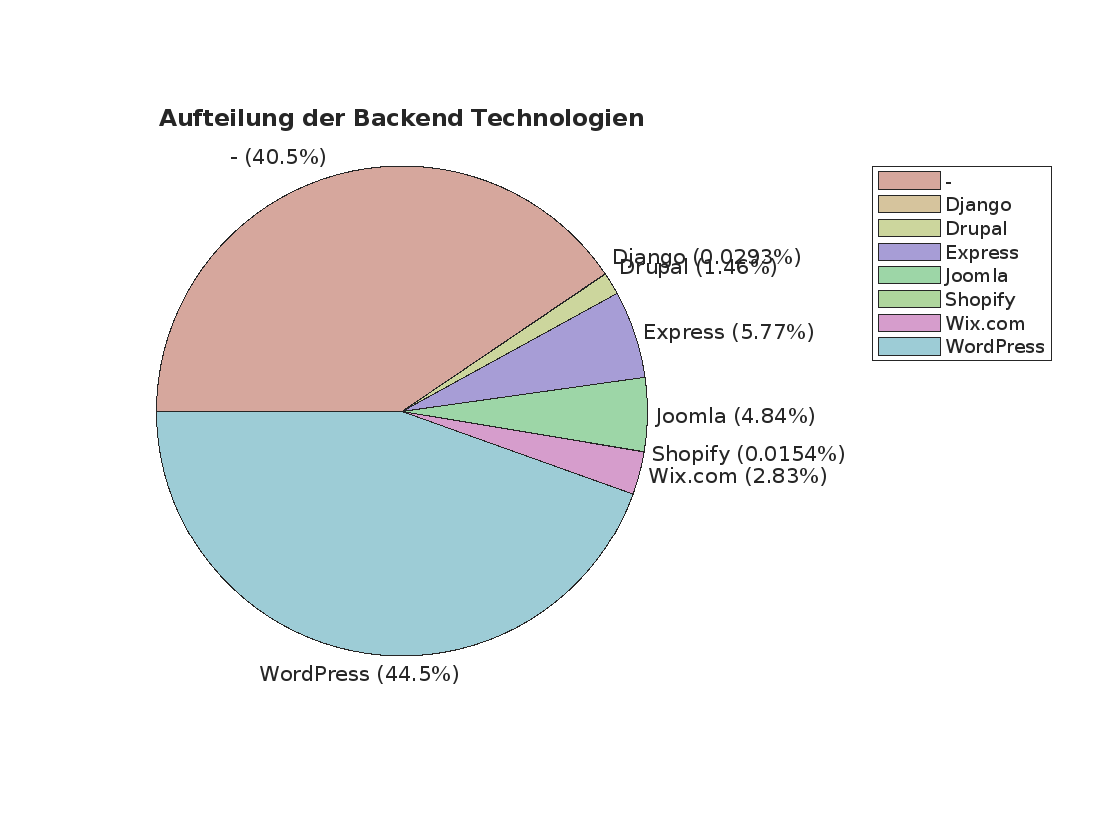
\includegraphics[width=1.0\linewidth]{matlab/pieBackendTechnologies.eps}
\caption{Verteilung der erkannten Backend Technologien in einem Tortendiagramm. (Quelle: Eigene Darstellung)}
\label{Abb1}
\end{figure}

\noindent Mit 44,5 \% ist WordPress der klare Marktführer. Weitere 40,5 \% der Webseiten konnten keiner spezifischen Backend-Technologie zugeordnet werden. Die restlichen 15 \% teilen sich andere Anbieter. Django und Shopify wurden jeweils nur bei einer Webseite erkannt.

\clearpage 

\subsection{Frontend Technologien}
\begin{figure}[htp]
\centering
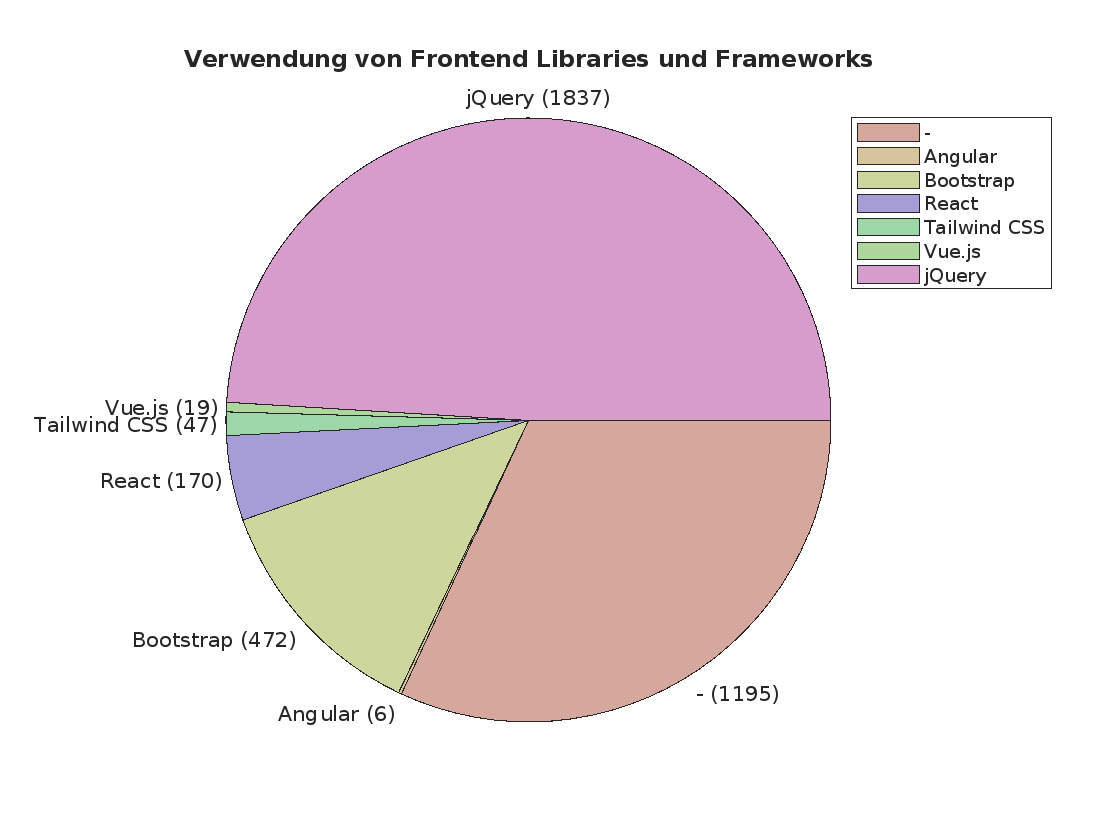
\includegraphics[width=1.0\linewidth]{matlab/pieLibraries.eps}
\caption{Verteilung der erkannten Frontend Libraries und Frameworks. (Quelle: Eigene Darstellung)}
\label{Abb2}
\end{figure}

\noindent Von den untersuchten Webseiten haben 1837 jQuery verwendet, gefolgt von 1195 Webseiten ohne namhafte Frontend-Frameworks oder Bibliotheken. Aufgrund des hohen Interesses an jQuery wurde auch die Version der verwendeten jQuery-Bibliothek untersucht. Ältere Versionen können erhebliche Sicherheitslücken und Performance-Einbußen darstellen.

\begin{figure}[hbp]
\centering
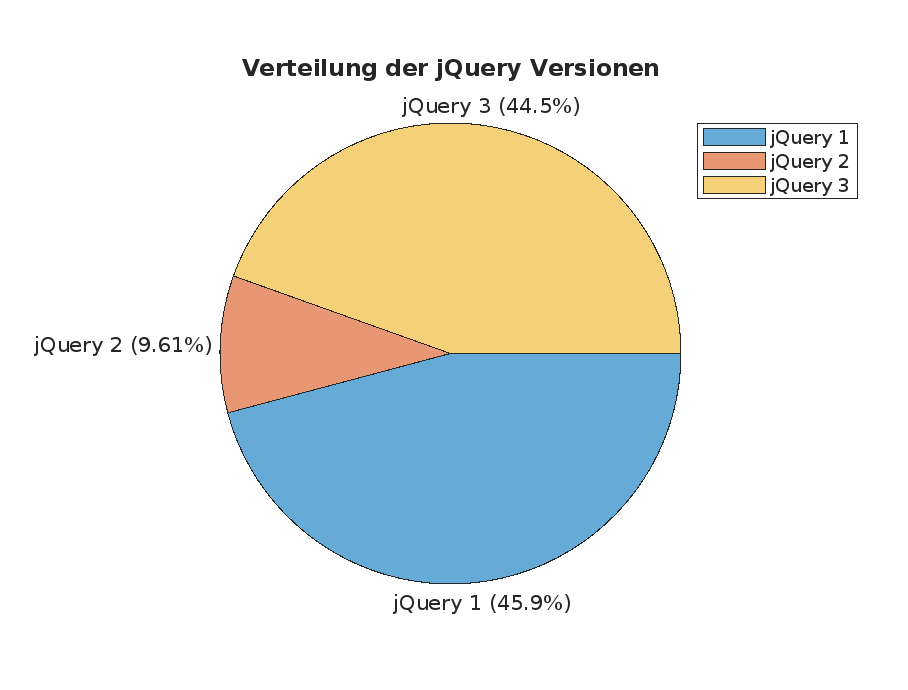
\includegraphics[width=1.0\linewidth]{matlab/pieJQuery.eps}
\caption{Verteilung der erkannten jQuery Versionen. (Quelle: Eigene Darstellung)}
\label{Abb3}
\end{figure}

% Mehr allgemeine Infos / Erkentnisse?
\clearpage 



\section{Bewertung der Hypothesen}
\noindent Der Schwerpunkt dieser Untersuchung lag auf dem Umweltaspekt und der damit verbundenen vergeudeten Energie durch lange Ladezeiten sowie den freigesetzten CO$_2$-Emissionen bei der Datenübertragung. Um die Ergebnisse der Ladezeiten und übertragenen Datenmengen zu normieren und in Relation zur Gesamtmenge der untersuchten Webseiten zu setzen, wurde folgende Formel entwickelt und angewendet:


\begin{align*}
T & \text{ - Ladezeit einer Webseite} \\
\bar{T} & \text{ - Durchschnittliche Ladezeit aller untersuchten Webseiten} \\
M & \text{ - Main-Thread-Arbeitszeit einer Webseite} \\
M_f & \text{ - Faktor der Main-Thread-Arbeitszeit, definiert als } \frac{M}{T} \\
E & \text{ - Energie Faktor} \\
C & \text{ - CO}_2\text{-Emissionen einer Webseite} \\
\bar{C} & \text{ - Durchschnittliche CO}_2\text{-Emissionen aller untersuchten Webseiten} \\
F & \text{ - CO}_2\text{-Faktor}
\end{align*}

\[
Impact = \sqrt{\left( \frac{T}{\bar{T}} \times M_f \right) \times \left( \frac{C}{\bar{C}} \right) \times EF}
\]

\noindent Die Kalkulation basiert auf der Annahme, dass während des Ladens einer Webseite das Gerät des Endnutzers weiterhin Strom verbraucht. Da österreichweit fast 90 \% des Website-Traffics von Mobilgeräten stammen  \cite{Stat21} und bei diesen oft über 70 \% des Energieverbrauchs allein auf den Bildschirm entfallen  \cite{Argos24}, wird die Ladezeit als Einsparpotenzial für Energie betrachtet. Da eine einzige Webseite potenziell mehrere Millionen Mal von verschiedenen Geräten aufgerufen werden kann, ist das Gesamteinsparpotenzial enorm, aber schwer abzuschätzen, wodurch eine Berücksichtigung der Gesamtanzahl verschiedenster Faktoren den Rahmen dieser Arbeit sprengen würde. \newline

\noindent Die normierte Ladezeit $L$ einer Webseite wird berechnet, indem sie durch den Durchschnitt aller Ladezeiten der untersuchten Webseiten $\bar{T}$ geteilt wird. Anschließend wird das Produkt aus Ladezeit und Main-Thread-Arbeitszeit $M_f$ gebildet, um den zusätzlichen Energieaufwand bei langer Main-Thread-Arbeitszeit zu berücksichtigen. Ähnlich werden die von CO2.js geschätzten CO$_2$-Emissionen $C$ durch den Durchschnitt aller Emissionen $\bar{C}$ geteilt und normiert. Danach werden die beiden normierten Werte – der Energiefaktor $E$ und der CO$_2$-Faktor $F$ – multipliziert und das Ergebnis wird quadriert, um Ausreißer zu glätten. Bei der Auswertung wurden diese Gewichte $EF$ jedoch nicht berücksichtigt, da zu viele externe Faktoren diese Gewichtung beeinflussen könnten. \newline

\noindent Weiter ist es schwer, ein pauschales Verhältnis zwischen der Energieverschwendung von Endgeräten und Datazentren festzulegen. Obwohl global gesehen nur 33 \% der CO$_2$-Emissionen auf Datazentren zurückzuführen sind  \cite{PoCo17}, variiert der Stromverbrauch zwischen den Programmiersprachen erheblich. Beispielsweise kann PHP bis zu 13,8 Mal mehr Strom verbrauchen als JavaScript und 29,3 Mal mehr als C  \cite{PrL17}  \cite{PrL20}. Auch Faktoren wie Browserwahl  \cite{EWCF20} und Verbindungsgeschwindigkeit sowie -qualität  \cite{5G21} spielen eine wesentliche Rolle in der Berechnung der tatsächlichen CO$_2$-Emissionen.

\clearpage 

\subsection{Bewertung der 1. Hypothese}

\begin{center}
\begin{quote}
\textit{Hypothese 1: Es besteht eine signifikante Korrelation zwischen der Verwendung moderner Web-Technologien und einer Reduzierung des Energieverbrauchs sowie der CO$_2$-Emissionen von Webseiten.}
\end{quote}
\end{center}

\noindent Um diese Hypothese zu überprüfen, wurde eine Kategorisierung aller untersuchten Webseiten nach ihren verwendeten Frontend- und Backend-Technologien durchgeführt. Zur quantitativen Bewertung dieser Hypothese wurden die CO$_2$-Emissionen und der zuvor erläuterte $Impact$ für jede Webseite berechnet und verglichen.

\begin{figure}[hbp]
\centering
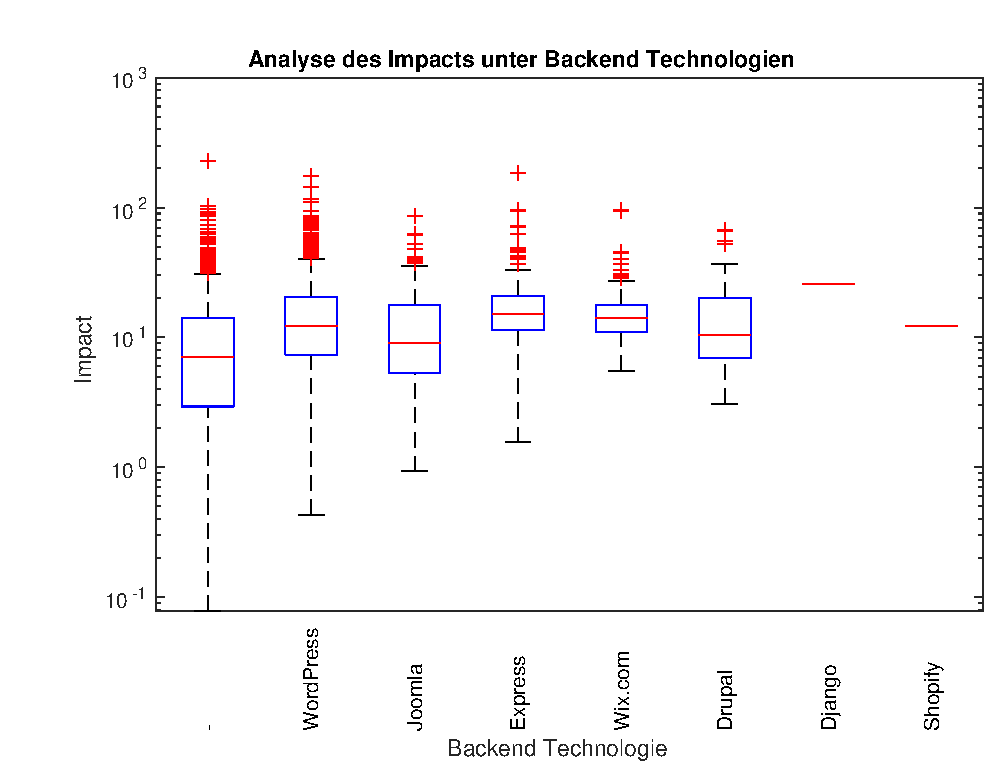
\includegraphics[width=1.0\linewidth]{matlab/distImpactbyBackend.eps}
\caption{Jeder Boxplot repräsentiert die Verteilung der CO$_2$-Emissionen für die jeweilige Backend Technologie: kein Backend (-), WordPress, Joomla, Express, Wix.com, Drupal, Django und Shopify. (Quelle: Eigene Darstellung)}
\label{Abb4}
\end{figure}

\noindent Die Analyse der Backend-Technologien offenbart bereits signifikante Unterschiede. Insbesondere zeigt WordPress das breiteste Spektrum an CO$_2$-Emissionen, was die Annahme stützt, dass die Nutzung von No-Code-Plattformen ohne entsprechendem Fachwissen zu erheblichen Performanceeinbußen führen kann.
\clearpage


\begin{figure}[htp]
\centering
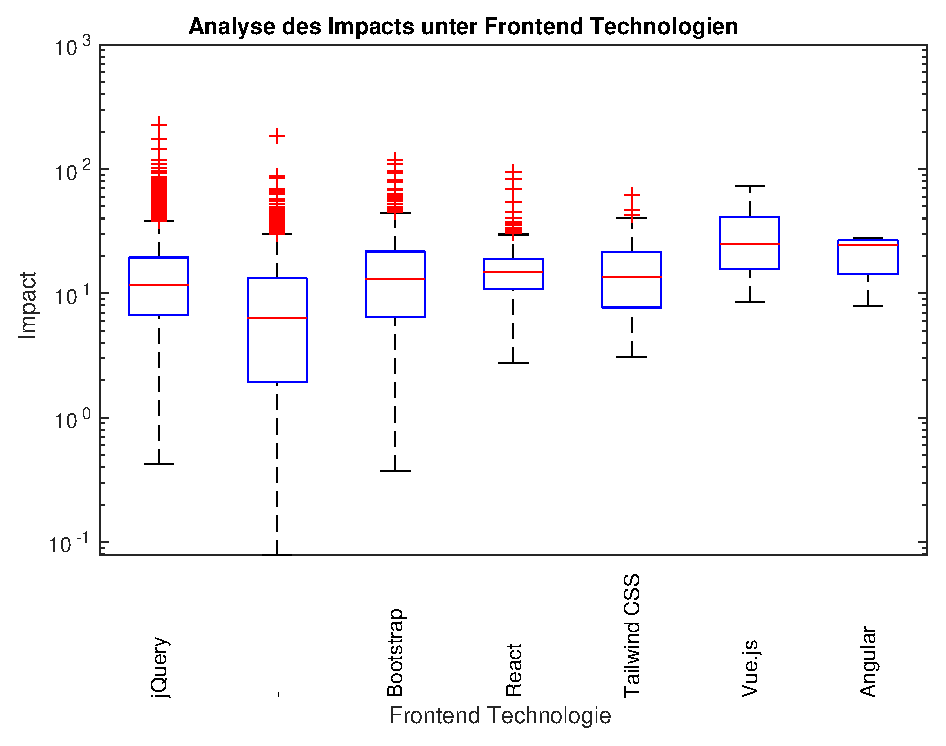
\includegraphics[width=1.0\linewidth]{matlab/distImpactbyFrontend.eps}
\caption{Jeder Boxplot repräsentiert die Verteilung der CO$_2$-Emissionen für die jeweilige Frontend Technologie. (Quelle: Eigene Darstellung)}
\label{Abb5}
\end{figure}

\noindent Bei der Analyse der Frontend-Technologien zeigte sich, dass sowohl die Nutzung als auch der Verzicht auf jQuery oder andere Bibliotheken die endgültige Performance nur geringfügig beeinflusst und zu großen Streuungen in den Daten führt. Vue.js schnitt jedoch am schlechtesten ab, da sowohl sein Median als auch seine Mittelwerte höher ausfielen als bei anderen Technologien. React hingegen zeigte die geringste Streuung der Mittelwerte und scheint eine deterministische Performance zu bieten. Es gab jedoch keine Ausreißer im Bereich niedriger Impact-Werte, während Webseiten mit jQuery, Bootstrap, oder ohne spezielle Frontend-Technologie manchmal bessere Ergebnisse lieferten als jede React-basierte Webseite.

\clearpage


\begin{figure}[htp]
\centering
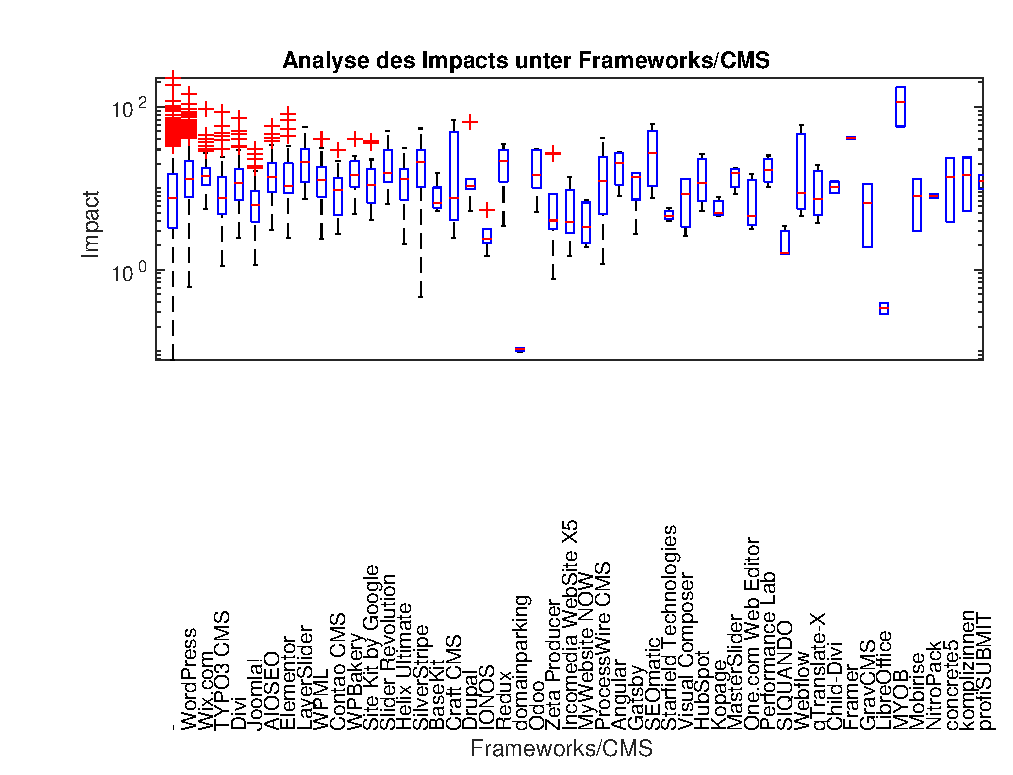
\includegraphics[width=1.0\linewidth]{matlab/distImpactbyFrameworksCMS.eps}
\caption{Jeder Boxplot repräsentiert die Verteilung der CO$_2$-Emissionen für die jeweiligen Frameworks/\ac{CMS}. (Quelle: Eigene Darstellung)}
\label{Abb6}
\end{figure}

\noindent Die Analyse der Frameworks und \ac{CMS} verdeutlicht deutliche Unterschiede in den erkannten Technologien. Während die größte Streuung bei jenen Webseiten zu beobachten war, bei denen keine Frameworks oder \ac{CMS} erkannt wurden, zeigten WordPress, Elementor, WPML und andere WordPress-bezogene Technologien eine Platzierung in den oberen Bereichen des Impact-Profils. Wix.com schnitt nur geringfügig besser ab als WPML, platzierte sich jedoch ebenfalls in einem hohen Bereich. Gute Platzierungen erreichen IONOS sowie einige weniger bekannte Technologien wie Zeta Producer, Incomedia Website und My Website NOW. \newline

\noindent Zusammenfassend lässt sich zur ersten Hypothese feststellen, dass trotz einer umfassenden Untersuchung, welche die CO$_2$-Emissionen in Bezug zu Ladezeiten und Main-Thread-Arbeitszeit setzte, keine signifikanten Unterschiede festgestellt werden konnten. Gewisse Unterschiede und Tendenzen in den erhobenen Daten waren erkennbar, jedoch nicht aussagekräftig genug, um als eindeutige Muster identifiziert zu werden. Diese Erkenntnis legt nahe, dass die alleinige Verwendung moderner Web-Technologien möglicherweise nicht ausreicht, um den Energieverbrauch und die CO$_2$-Emissionen signifikant zu reduzieren.

\clearpage


\subsection{Überprüfung von Hypothese 2}

\begin{center}
\begin{quote}
\textit{Hypothese 2: Webseiten, die für Performance und Effizienz optimiert sind (z.B. durch die Minimierung des Datenverkehrs und effiziente Ressourcennutzung), haben im Vergleich zu weniger optimierten Webseiten einen geringeren ökologischen Fußabdruck..}
\end{quote}
\end{center}

\noindent Um diese Hypothese zu überprüfen, wurde der Lighthouse Score als Indikator für eine optimierte Webseite herangezogen und mit den geschätzten CO$_2$-Emissionen verglichen. 

\begin{figure}[htp]
\centering
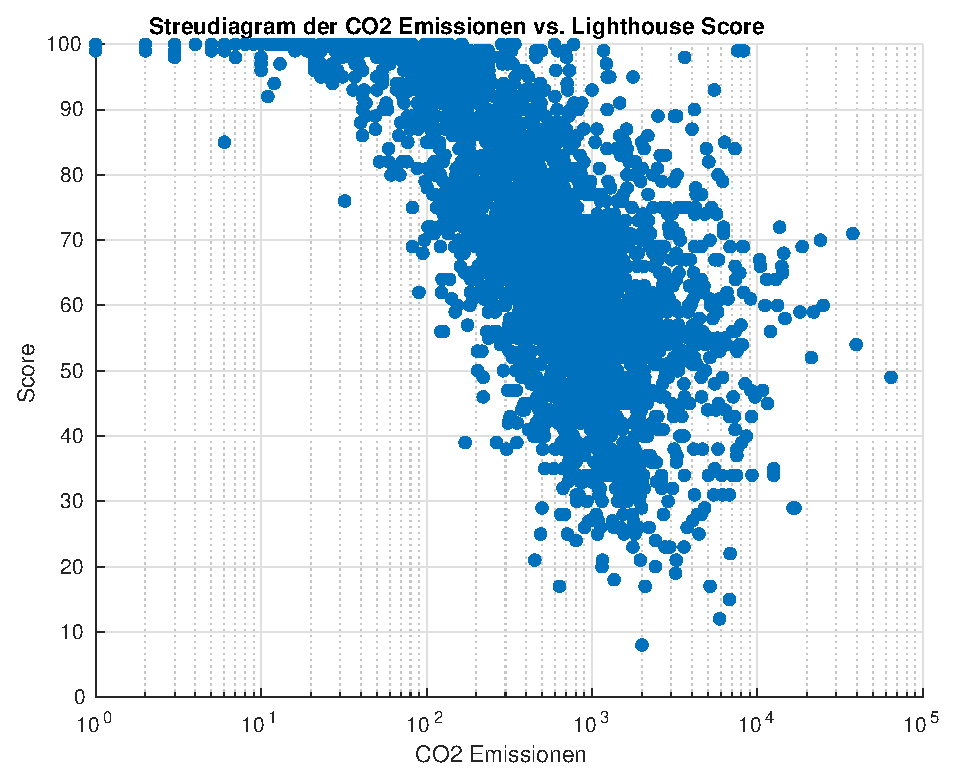
\includegraphics[width=1.0\linewidth]{matlab/scatterCO2vsScore.eps}
\caption{Verteilung der CO$_2$ Emissionen gegenüber dem Lighthouse Score. (Quelle: Eigene Darstellung)}
\label{Abb7}
\end{figure}

\noindent Der eindeutige Abwärtstrend zeigt, dass mit einem sinkenden Lighthouse Score die CO$_2$-Emissionen ansteigen. Somit wird die zweite Hypothese bestätigt.

\clearpage


% ------------------------------------------------------------------------------------------
% KAPITEL 4 - Diskussion - 15%
\chapter{Diskussion}

\section{Ergebnisinterpretation}

Die in der Analyse dargelegten Daten offenbaren die Unterschiede zwischen den verschiedenen Backend- und Frontend-Technologien sowie den verwendeten Frameworks und \ac{CMS} bezüglich ihres Einflusses auf CO$_2$-Emissionen und Performance. WordPress, als Beispiel für eine No-Code-Lösung, weist eine breite Spanne an CO$_2$-Emissionen auf. Dies deutet darauf hin, dass der Einsatz solcher Technologien ohne tiefgreifendes Fachwissen zu Performancenachteilen führen kann, die wiederum erhöhte Umweltauswirkungen nach sich ziehen. Diese Erkenntnis stützt die Vermutung, dass die Wahl der Technologie und das Wissen über ihre effiziente Nutzung entscheidend sind, um umweltfreundlichere Web-Lösungen zu schaffen.\newline

\noindent Bei den Frontend-Technologien zeigt sich, dass weder die Nutzung noch der Verzicht auf Bibliotheken wie jQuery die Performance wesentlich beeinflussen, was auf eine hohe Variabilität in der Implementierung hindeutet. Vue.js zeigte im Vergleich zu anderen Technologien schlechtere Leistungswerte, während React konsistentere Mittelwerte aufwies, jedoch ohne signifikante Spitzen in umweltfreundlichen Bereichen. Dies könnte darauf hinweisen, dass trotz der Vorhersehbarkeit in der Performance durch die Nutzung von React, die Optimierungsmöglichkeiten möglicherweise noch nicht vollständig ausgeschöpft werden, oder die Bibliothek ein gewisses Maß an Grund-Leistung benötigt.\newline

\noindent Die Analyse der Frameworks und \ac{CMS} zeigt, dass Technologien, die auf WordPress basieren, tendenziell höhere CO$_2$-Emissionen verursachen, was deren Platzierung in den oberen Bereichen der Impact-Skala erklärt. Dies unterstreicht die Notwendigkeit für Entwickler, bei der Wahl und Implementierung dieser Technologien sorgfältig zu überlegen, wie sie den Energieverbrauch minimieren können.

\section{Bedeutung der Ergebnisse}
Die Ergebnisse dieser Studie sind besonders relevant für Webentwickler und -designer, sowie Entscheidungsträger in der Technologiebranche. Sie verdeutlichen, dass die bloße Auswahl moderner Web-Technologien nicht ausreichend ist, um den Energieverbrauch und die CO$_2$-Emissionen signifikant zu reduzieren. Vielmehr ist ein tiefes Verständnis der Funktionsweise und eine optimierte Implementierung dieser Technologien erforderlich. Zudem zeigt der klare Zusammenhang zwischen niedrigeren Lighthouse Scores und höheren CO$_2$-Emissionen, wie wichtig eine umfassende Optimierung für die umweltfreundliche Webentwicklung ist.

\section{Empfehlungen und Best Practices}

Auf Grundlage der Ergebnisse lassen sich mehrere Empfehlungen formulieren:

\begin{itemize}
    \item Optimierung der Codebasis: Entwickler sollten Techniken wie Lazy Loading, Tree-Shaking und Code Minification anwenden, um den Datenverkehr und die Ladezeiten zu minimieren.
    \item Bewusste Technologiewahl: Die Auswahl von Technologien sollte nicht nur auf Basis der Funktionalität, sondern auch unter Berücksichtigung ihres Potenzials zur Minimierung des ökologischen Fußabdrucks erfolgen.
    \item Fortbildung und Bewusstseinsbildung: Es ist essenziell, dass Entwickler und Designer in den Prinzipien der umweltfreundlichen Webentwicklung geschult werden.
\end{itemize}

\section{Limitationen der Studie}
\subsection{Technische und methodische Limitationen}

\subsubsection{Anpassung der Analysemethoden}
Im Verlauf der Entwicklung des Webcrawlers und der Analysemethoden wurden mehrere Anpassungen vorgenommen, um die Genauigkeit der Ergebnisse zu maximieren. Trotz dieser Bemühungen stieß man auf Grenzen bei der Erfassung bestimmter Daten, insbesondere bei Webseiten, die ihre verwendeten Technologien effektiv verbergen. Diese Limitation führt zu potenziellen Verzerrungen in den gesammelten Daten, da nicht alle relevanten Informationen erfasst werden konnten.

\subsubsection{Hardware-Limitationen und Performance-Ergebnisse}
Nach dem ersten Probelauf des Crawlers wurde festgestellt, dass die verwendete Hardware anfällig für Überhitzung war, was die Performance des Crawlers beeinträchtigte. Insbesondere die Ladezeiten der analysierten Webseiten waren teilweise doppelt so hoch im Vergleich zu Prüfdurchläufen, in denen die Hardware abgekühlt war. Als Lösungsansatz wurde der Crawling-Prozess angepasst, indem die Menge der untersuchten Webseiten in 10er Chunks aufgeteilt wurde. Nach jeweils zehn analysierten Webseiten erfolgte eine Wartezeit von 30 Sekunden, um die Hardware abkühlen zu lassen. Diese Maßnahme verbesserte die Zuverlässigkeit der Performance-Ergebnisse, führte jedoch zu einer Verlängerung der Gesamtdauer des Crawling-Prozesses.

\subsubsection{Memory Leaks in der Lighthouse Bibliothek}
Eine weitere technische Herausforderung stellten Memory Leaks in der verwendeten Lighthouse Bibliothek dar. Wenn der Crawler über einen längeren Zeitraum lief, füllte sich der RAM zunehmend, was zu Performance-Einbußen führte. Als Gegenmaßnahme wurde der Crawler in einem neuen Terminalfenster gestartet, um jeweils zehn Webseiten zu testen. Das \hyperref[code:run]{Bash-Script} findet sich im \hyperref[chap:appendix]{Anhang}. Nach Abschluss schloss sich das Fenster automatisch, und nach einer Wartezeit von 30 Sekunden öffnete sich ein neues Fenster für den nächsten Durchlauf. Diese Maßnahme ermöglichte es, den RAM auf Betriebssystemebene zu entleeren und die Leistungsfähigkeit des Crawlers zu erhalten. Allerdings erhöhte diese Lösung die Komplexität des Crawlers.

\subsection{Herausforderungen bei der Datensammlung}

\subsubsection{Versteckte Technologien}
Wie bereits erwähnt, verwenden manche Webseitenbetreiber Techniken, um ihre eingesetzten Technologien zu verbergen. Die Gründe hierfür können vielfältig sein, von der Absicht, sich vor potenziellen Sicherheitsrisiken zu schützen, bis hin zu dem Wunsch, proprietäre Informationen nicht preiszugeben. Die Identifizierung der verwendeten Technologien war in diesen Fällen oft schwierig, was die Vollständigkeit der gesammelten Daten beeinträchtigte.

\subsubsection{Blockierung der Crawler-Software}
Eine weitere Herausforderung stellte die Blockierung des automatisierten Zugriffs durch einige Webseiten dar. Um dieses Hindernis zu überwinden, wurde der User-Agent-Header des Crawlers angepasst, um die Erkennung als automatisierte Software zu umgehen und stattdessen einen normalen Besucher vorzutäuschen. Der beschriebene \hyperref[code:useragent]{User-Agent-Header} findet sich im \hyperref[chap:appendix]{Anhang}. Diese Anpassung war notwendig, um Zugang zu den Webseiten zu erhalten und relevante Daten sammeln zu können.

\subsubsection{Variabilität der Server-Performance}
Die Performance von Webseiten ist abhängig von externen Faktoren, die außerhalb der Kontrolle des Forschungsprojekts liegen. Beispielsweise kann die Tageszeit einen erheblichen Einfluss auf die Serverauslastung haben, was zu Schwankungen in den Ladezeiten und damit zu Verzerrungen in den Performance-Ergebnissen führen kann. Um diesen Variablen Rechnung zu tragen, wurde beschlossen, die Datensammlung hauptsächlich nachts durchzuführen, wenn die Netzwerkauslastung generell niedriger ist. Zusätzlich wurden die Daten von jeder Webseite insgesamt dreimal gesammelt, um temporäre Schwankungen zu berücksichtigen. Für die Analyse wurden dann jeweils die besten der drei Ergebnisse verwendet, um die optimale Performance der Server widerzuspiegeln. Diese Strategie sollte dazu beitragen, die Zuverlässigkeit der gesammelten Daten zu erhöhen, führte jedoch zu einem erheblich höheren Zeitaufwand für die Datensammlung.


\section{Schlussfolgerungen}

Die in dieser Arbeit durchgeführte Analyse hat wichtige Erkenntnisse über den Zusammenhang zwischen der Nutzung von Web-Technologien und deren Einfluss auf die CO$_2$-Emissionen sowie den Energieverbrauch geliefert. Die Untersuchung verschiedener Backend- und Frontend-Technologien, Frameworks und \ac{CMS} hat gezeigt, dass die Auswahl und Implementierung der Technologien einen deutlichen Einfluss auf die ökologische Nachhaltigkeit von Webseiten haben kann. \newline

\noindent Trotz der beobachteten Unterschiede und Tendenzen konnte Hypothese 1, welche eine signifikante Korrelation zwischen der Nutzung moderner Technologien und einer Reduzierung von CO$_2$-Emissionen sowie Energieverbrauch postulierte, nicht eindeutig bestätigt werden. Dies deutet darauf hin, dass die bloße Verwendung neuerer oder populärer Technologien nicht automatisch zu einer verbesserten ökologischen Effizienz führt. Vielmehr ist es die Art und Weise, wie diese Technologien implementiert und optimiert werden, die entscheidend ist.\newline

\noindent Die Bestätigung der zweiten Hypothese, dass Webseiten mit optimierter Performance auch geringere CO$_2$-Emissionen aufweisen, unterstreicht die Bedeutung einer durchdachten und umfassenden Optimierung. Hierbei spielen sowohl technische Aspekte wie die Minimierung von Datenverkehr und effiziente Ressourcennutzung als auch die Auswahl der richtigen Technologien eine entscheidende Rolle.\newline

\noindent Diese Erkenntnisse legen nahe, dass eine umfassende Ausbildung und Sensibilisierung von Webentwicklern und -designern hinsichtlich der ökologischen Auswirkungen ihrer Arbeit von großer Bedeutung sind. Zudem wird deutlich, dass nachhaltige Webentwicklung ein fortlaufender Prozess ist, der sowohl fortgeschrittene technische Fähigkeiten als auch ein tiefes Verständnis für die Wechselwirkungen zwischen Technologie, Performance und Umwelt erfordert.\newline

\noindent Abschließend lässt sich festhalten, dass die Entwicklung von umweltfreundlicheren Webanwendungen eine gemeinschaftliche Anstrengung erfordert, die über die Grenzen einzelner Technologien hinausgeht und eine integrierte Betrachtung von Design, Entwicklung und Optimierung erfordert. Die Ergebnisse dieser Arbeit bieten eine wertvolle Grundlage für zukünftige Forschungen in diesem Bereich und für die Praxis der Webentwicklung, die zunehmend auf Nachhaltigkeit ausgerichtet sein muss.



\clearpage  
















%%%%%%%%%%%%%%%%%%%%%%%%%%%%%%%%%%%%%%%%%%%%%%%%%%%%%%%%%%%%%%%%%% Hier beginnen die Verzeichnisse.
\clearpage                                                       % Beginne neue Seite

\printbib                                                        % Literaturverzeichnis LaTeX-Zitier-Standard
%\printbib{Literatur}                                             % Literaturverzeichnis FH-Zitier-Standard
\clearpage

\listoffigures                                                   % Abbildungsverzeichnis
\clearpage

\listoftables                                                    % Tabellenverzeichnis
\clearpage

\listoflistings                                                  % Quellcodeverzeichnis
\clearpage

\phantomsection
\addcontentsline{toc}{chapter}{\listacroname}
\chapter*{\listacroname}
\begin{acronym}[XXXXX]
    \acro{IKT}[IKT]{Informations- und Kommunikations-Technologie}
    \acro{LCP}[LCP]{Largest Contentful Paint}
    \acro{TTI}[TTI]{Time to Interactive}
    \acro{CMS}[CMS]{Content Management System}
    \acro{KMU}[KMU]{kleine und mittlere Unternehmen}
    \acro{CDN}[CDN]{Content Delivery Network}
\end{acronym}
%%%%%%%%%%%%%%%%%%%%%%%%%%%%%%%%%%%%%%%%%%%%%%%%%%%%%%%%%%%%%%%%%% Hier beginnt der Anhang.
\clearpage
\appendix

\chapter{QR Code zum GitHub-Repository}
\label{chap:appendix}

\begin{figure}[!htbp]
\centering
\includegraphics[width=0.5\linewidth]{PICs/frame}
\caption{QR-Code zum GitHub-Repository dieser Arbeit. Enthalten sind der Quellcode für den Crawler, der Quellcode dieser Arbeit in LaTeX, der Quellcode der MATLAB-Grafiken und die Ergebnisse der Analyse als CSV-Datei. (Quelle: Eigene Darstellung durch qr-code-generator.com)}\label{Abb2}
\end{figure}

\clearpage

\chapter{Webcrawler und MATLAB Quellcode}
\label{chap:appendix}

\begin{listing}[htbp]
\begin{minted}[
    frame=single,
    framesep=2mm,
    baselinestretch=1.2,
    bgcolor=white,
    fontsize=\footnotesize,
    linenos
    ]{bash}
#!/bin/bash

CHUNK_SIZE=10
WAIT_DURATION=10
PAUSE_DURATION=30

TOTAL_URLS=3284
let TOTAL_CHUNKS=($TOTAL_URLS+$CHUNK_SIZE-1)/$CHUNK_SIZE

local_arg=""

for ((i=1; i<=$#; i++)); do
    if [ "${!i}" == "--local" ]; then
        echo "Running in local mode"
        let next_index=i+1
        local_arg="${!next_index}"
        break
    fi
done

for (( i=0; i<$TOTAL_CHUNKS; i++ ))
do
    let START=$i*$CHUNK_SIZE
    let END=($i+1)*$CHUNK_SIZE-1

    konsole --new-tab -e "bash -c 'node index.js $START $END $local_arg'" &
    while [ ! -f "complete.txt" ]; do sleep $WAIT_DURATION; done

    echo "done found"
    
    rm complete.txt

    sleep $PAUSE_DURATION
done
\end{minted}
\caption{\textbf{run.sh} - Startet die Datensammlung. Arbeitet sich in 10er Chunks durch und wartet 30 Sekunden zwischen den Durchläufen.}
\label{code:run}
\end{listing}


\begin{listing}[htbp]
\begin{minted}[
    frame=single,
    framesep=2mm,
    baselinestretch=1.2,
    bgcolor=white,
    fontsize=\footnotesize,
    linenos
    ]{javascript}
const response = await axios.get(websiteUrl, {
    headers: {
        'User-Agent': 'Mozilla/5.0 (X11; Linux x86_64; rv:123.0) 
            Gecko/20100101 Firefox/123.0',
        'Accept-Language': 'en-US,en;q=0.9',
        'Accept': 'text/html,application/xhtml+xml,
            application/xml;q=0.9,image/avif,image/webp,*/*;q=0.8',
        'Accept-Encoding': 'gzip, deflate, br',
        'Referer': 'https://www.google.com/',
        'Cache-Control': 'no-cache',
    }
});
\end{minted}
\caption{\textbf{User-Agent-Header} zur Umgehung der Crawler-Blockierung}
\label{code:useragent}
\end{listing}


\begin{listing}[htbp]
\begin{minted}[
    frame=single,
    framesep=2mm,
    baselinestretch=1.2,
    bgcolor=white,
    fontsize=\footnotesize,
    linenos
    ]{matlab}
data =  readtable('./data/lighthouse_data4_full.csv');

% Initialize a map to hold the count for each major version of jQuery
jqueryVersionCount = containers.Map('KeyType', 'char', 'ValueType', 'double');

% Iterate through each row in the data
for i = 1:height(data)
    % Split the technologies by comma for the current row and trim spaces
    techs = strtrim(strsplit(data.libraries{i}, ','));
    % For each technology in the current row
    for j = 1:length(techs)
        tech = techs{j};
        
        % Check if the technology starts with 'jQuery'
        if startsWith(tech, 'jQuery')
            % Regular expression to extract version numbers
            versionPattern = '^jQuery\s+(\d+)';
            tokens = regexp(tech, versionPattern, 'tokens');
            if ~isempty(tokens)
                % Build the grouped version name (e.g., 'jQuery 3')
                majorVersion = tokens{1}{1};
                groupedVersionName = ['jQuery ', majorVersion];
                
                % Count the occurrences
                if isKey(jqueryVersionCount, groupedVersionName)
                    jqueryVersionCount(groupedVersionName) = 
                        jqueryVersionCount(groupedVersionName) + 1;
                else
                    jqueryVersionCount(groupedVersionName) = 1;
                end
            end
        end
    end
end

% Extract the technology names and their respective counts
techNames = keys(jqueryVersionCount);
techCounts = zeros(length(techNames), 1);

% Accumulate the counts for each technology
for i = 1:length(techNames)
    techCounts(i) = jqueryVersionCount(techNames{i});
end

% Plotting the pie chart
piechart(techCounts,techNames,LabelStyle="namepercent", LegendVisible="on", StartAngle="90");
title('Verteilung der jQuery versionen');

print -depsc pieJQuery.eps
\end{minted}
\caption{\textbf{pieJQuery.m} - Beispiel der Erstellung eines Tortendiagramms}
\end{listing}



\begin{listing}[htbp]
\begin{minted}[
    frame=single,
    framesep=2mm,
    baselinestretch=1.2,
    bgcolor=white,
    fontsize=\footnotesize,
    linenos
    ]{matlab}
% Load the CSV file
data =  readtable('./data/lighthouse_data4_impact.csv');

% Initialize arrays to hold CO2 values and their corresponding technologies
allCO2Values = []; allTechs = {};

% Iterate through each row in the data
for i = 1:height(data)
    % Split the technologies by comma for the current row and trim spaces
    techs = strtrim(strsplit(data.frameworks{i}, ','));
    % For each technology in the current row
    for j = 1:length(techs)
        tech = techs{j};
        allCO2Values = [allCO2Values; data.impact(i)];
        allTechs = [allTechs; {tech}];
    end
end

% Calculate the frequency of each technology
[uniqueTechs, ~, idx] = unique(allTechs);
techCounts = accumarray(idx, 1);

% Sort the technologies by frequency in descending order
[~, sortIdx] = sort(techCounts, 'descend');
sortedTechs = uniqueTechs(sortIdx);
sortedCO2Values = []; sortedAllTechs = {};

% Populate the new arrays according to the sorted order of technologies
for i = 1:length(sortedTechs)
    tech = sortedTechs{i};
    techIndices = strcmp(allTechs, tech);
    sortedCO2Values = [sortedCO2Values; allCO2Values(techIndices)];
    sortedAllTechs = [sortedAllTechs; allTechs(techIndices)];
end

boxplot(sortedCO2Values, sortedAllTechs, 'LabelOrientation', 'inline', 
    'Whisker', 1.5);
ylabel('Impact');
xlabel('Frameworks/CMS');
title('Analyse des Impacts unter Frameworks/CMS');
xtickangle(45);
set(gca, 'YScale', 'log');
xlim([0, 50]);

print -depsc distImpactbyFrameworksCMS.eps
\end{minted}
\caption{\textbf{distImpactByFrameworksCMS.m} - Beispiel einer Funktion zur Erstellung der Boxplot Grafiken}
\end{listing}


\begin{listing}[htbp]
\begin{minted}[
    frame=single,
    framesep=2mm,
    baselinestretch=1.2,
    bgcolor=white,
    fontsize=\footnotesize,
    linenos
    ]{matlab}
% Load the CSV file
data =  readtable('./data/lighthouse_data4_impact.csv');

% Initialize arrays to hold CO2 values and their corresponding scores
xValues = [];
yValues = [];
allTechs = {};

% Iterate through each row in the data
for i = 1:height(data)
    % Split the technologies by comma for the current row and trim spaces
    techs = strtrim(strsplit(data.frameworks{i}, ','));
    % For each technology in the current row
    for j = 1:length(techs)
        tech = techs{j};
        % Append the CO2 and score values to the xValues and yValues arrays
        xValues = [xValues; data.CO2WithGreenHosting(i)];
        yValues = [yValues; data.score(i)];
        allTechs = [allTechs; {tech}];
    end
end

% Plot the scatter diagram
scatter(xValues, yValues, 'filled');
xlabel('CO2 Emissionen');
ylabel('Lighthouse Score');
title('Streudiagram der CO2 Emissionen vs. Lighthouse Score');
grid on;  % Turn on the grid
ax = gca; % Get current axes
ax.XAxis.Exponent = 0; % Prevent scientific notation on x-axis
ax.YAxis.Exponent = 0; % Prevent scientific notation on y-axis

set(gca, 'XScale', 'log');

print -depsc scatterCO2vsScore.eps
\end{minted}
\caption{\textbf{scatterCO2vsScore.m} - Erstellung des Streudiagrams für CO$_2$-Emissionen und Lighthouse Score}
\end{listing}


\clearpage
%\chapter{Anhang B}
\end{document}
%%%%%%%%%%%%%%%%%%%%%%%%%%%%%%%%%%%%%%%%%%%%%%%%%%%%%%%%%%%%%%%%%% Ende des Inhalts